\documentclass[xcolor=table]{beamer}
\usetheme{uic}
\usepackage{minted}
\usepackage{amsfonts,amsmath,oldgerm,algorithmic,algorithm}
\usepackage[font=small,labelfont=bf]{caption} % Required for specifying captions to tables and figures
\usepackage{tcolorbox}
\tcbuselibrary{listings,skins}
\usepackage{alltt,xcolor}
\usepackage{hyperref}
\usepackage{comment}
\usepackage{amsthm}
\usepackage[spanish]{babel}


\lstdefinestyle{mystyle}{
language=C
}

\newtcblisting{mylisting}[2][]{
    arc=0pt, outer arc=0pt,
    listing only, 
    listing style=mystyle,
    title=#2,
    #1
}


\newcommand{\hrefcol}[2]{\textcolor{uihteal}{\href{#1}{#2}}}
\newcommand{\testcolor}[1]{\colorbox{#1}{\textcolor{#1}{test}}~\texttt{#1}}

% Please see Section 18.1 of Beamer User Guide for all the options \usefonttheme provides
\usefonttheme[onlymath]{serif}
% \usefonttheme{serif} % use this if you would like Serif font throughout (and not just for math)

\title{Fundamentos de Inteligencia Artificial}
\titlebackground{images/etsiinformatica3.jpeg}
% an asterisk will split the background:
% \titlebackground*{images/uic_seo.jpg}
\subtitle{Búsquedas No informadas}

\author{\href{mailto:jmmontes@uma.es}{José A. Montenegro}}
\date{\today}

%https://aima.cs.berkeley.edu/algorithms.pdf


\begin{document}

\newtheorem{mydef}{Definición}[section] % Añade [section] para que se reinicie en cada sección
\maketitle

% default is no footline, but page numbers are incredibly useful for the audience to ask questions later
\footlinecolor{uicblue}

%%%%%%%%%%%%%%%%%%%%%%%%%%%%%%%%%%%%%%%%%%%%%%%%%%%
%%%%%%%%%%%%%%%%%%%%%%%%%%%%%%%%%%%%%%%%%%%%%%%%%%%
%%%%%%%%%%%%%%%%%%%%%%%%%%%%%%%%%%%%%%%%%%%%%%%%%%%
%%%%%%%%%%%%%%%%%%%%%%%%%%%%%%%%%%%%%%%%%%%%%%%%%%%
%%%%%%%%%%%%%%%%%%%%%%%%%%%%%%%%%%%%%%%%%%%%%%%%%%%
%%%%%%%%%%%%%%%%%%%%%%%%%%%%%%%%%%%%%%%%%%%%%%%%%%%


%%%%%%%%%%%%%%%%%%%%%%%%%%%%%%%%%%%%%%%%%%%%%%%%%%%
%%%%%%%%%%%%%%%%%%%%%%%%%%%%%%%%%%%%%%%%%%%%%%%%%%%
%%%%%%%%%%%%%%%%%%%%%%%%%%%%%%%%%%%%%%%%%%%%%%%%%%%
%%%%%%%%%%%%%%%%%%%%%%%%%%%%%%%%%%%%%%%%%%%%%%%%%%%
%%%%%%%%%%%%%%%%%%%%%%%%%%%%%%%%%%%%%%%%%%%%%%%%%%%
%%%%%%%%%%%%%%%%%%%%%%%%%%%%%%%%%%%%%%%%%%%%%%%%%%%


\begin{frame}{Contenido}
\tableofcontents
\end{frame}

%%%%%%%%%%%%%%%%%%%%%%%%%%%%%%%%
%%%%%%%%%%%%%%%%%%%%%%%%%%%%%%%%
%SECCION %%%%%%%%%%%%%%%%%%%%%%%%%%%%%%%
%%%%%%%%%%%%%%%%%%%%%%%%%%%%%%%%
%%%%%%%%%%%%%%%%%%%%%% 

\begin{chapter}[images/etsiinformatica4.png]{uicblue}{Búsqueda de Soluciones}
\end{chapter}

\section{Búsqueda de Soluciones}
%%%%%%%%%%%%%%%%%%%%%%%%%%%%%%%%
%%%%%%%%%%%%%%%%%%%%%%%%%%%%%%%%
%%%%%%%%%%%%%%%%%%%%%%%%%%%%%%%%

\begin{frame} \frametitle{Resolución problema} \footnotesize

\begin{itemize}
\item  Normalmente el espacio de estados generado por el estado inicial y la función sucesor es representado por un \textbf{árbol de búsqueda}.
\item  Cuando un estado es alcanzable por varios caminos tendremos un \textbf{grafo de búsqueda}. 
\end{itemize}


\begin{figure}
\includegraphics[scale=0.45]{./img/nodoArbol}
\end{figure}

\end{frame} 

%%%%%%%%%%%%%%%%%%%%%%%%%%%%%%%%

\begin{frame} \frametitle{Resolución problema} \footnotesize

\begin{itemize}
\item  El algoritmo general sería comenzando en la raíz, escoge, comprueba y expande hasta que encuentra una solución o no existen más estados para expandir.
\end{itemize}


\begin{figure}
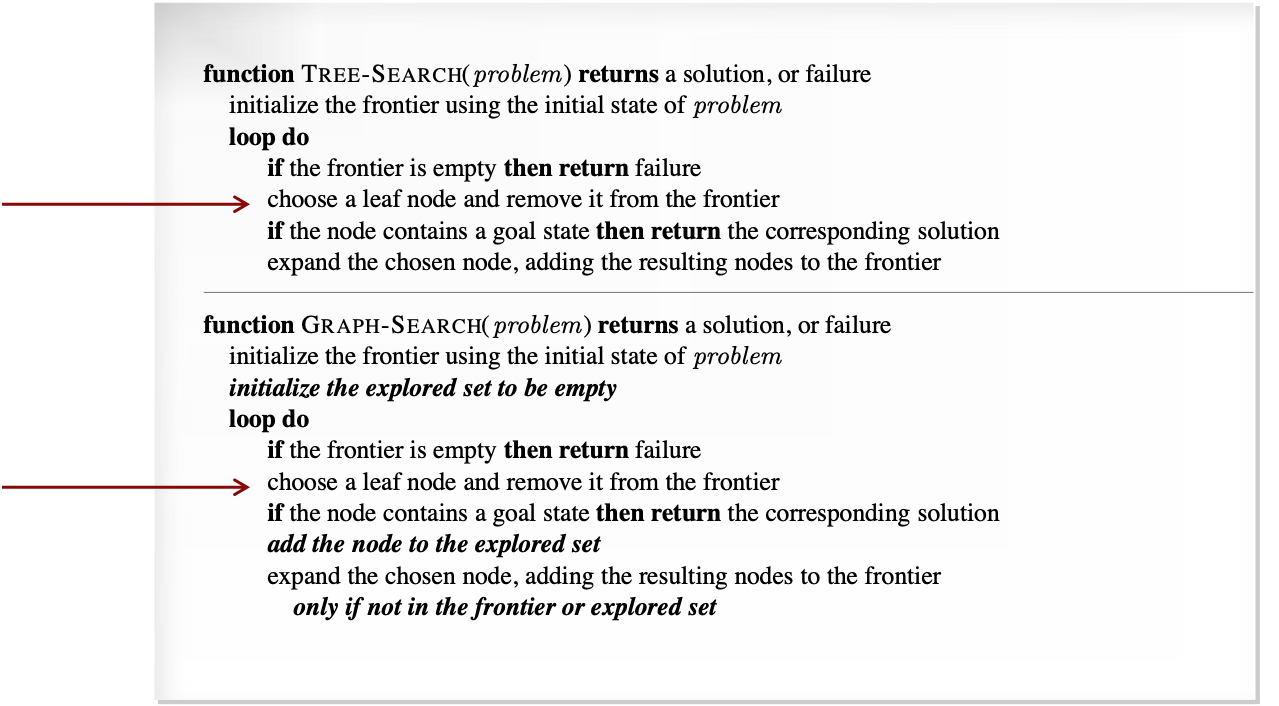
\includegraphics[scale=0.42]{./img/Arbol-Grafo}
\end{figure}

\end{frame} 

%%%%%%%%%%%%%%%%%%%%%%%%%%%%%%%%

\begin{frame} \frametitle{Resolución problema} \footnotesize

\begin{description}
\item [Frontera]: La colección (conjunto) de nodos (nodos hoja) que se generan pero no se ha expandido. 
\begin{itemize}
\item La estrategia de búsqueda será una función que seleccione del conjunto el siguiente nodo a expandir.
\end{itemize}
\end{description}


\begin{figure}
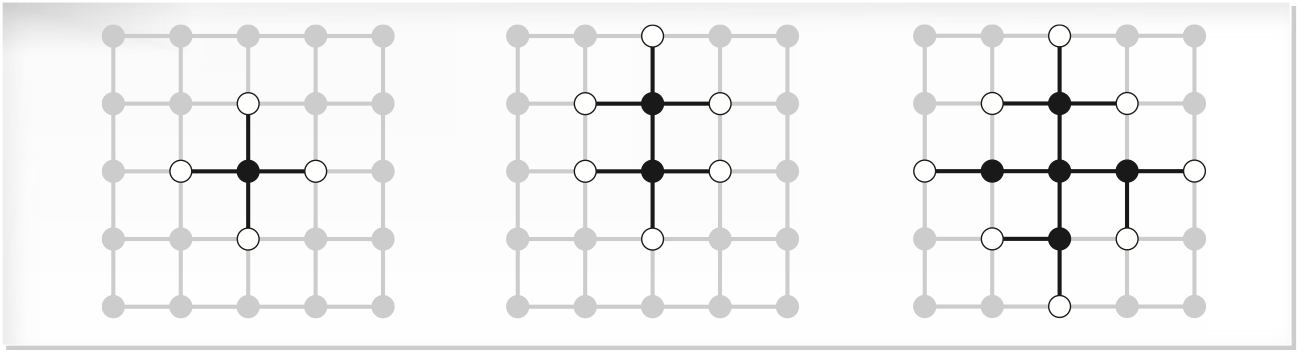
\includegraphics[scale=0.45]{./img/Frontera}
\end{figure}

\end{frame} 
%%%%%%%%%%%%%%%%%%%%%%%%%%%%%%%%

\begin{frame} \frametitle{Rendimiento de la resolución} \footnotesize

\begin{description}
\item [Completitud]: Garantizado algoritmo encuentra solución cuando existe.
\item [Optimización]: Encuentra la estrategia la solución óptima.
\item [Complejidad en tiempo]: Cuanto tarda en encontrar la solución.
\item [Complejidad en espacio]: Cuanta memoria necesita para el funcionamiento de la búsqueda.

\item [Eficiencia]: 
	\begin{itemize}
		\item Coste de la búsqueda, complejidad en tiempo y también uso memoria. 
		\item Coste total, coste de la búsqueda y coste del camino solución encontrado.
		\end{itemize}
\end{description}


\end{frame} 

\section{Búsquedas No informadas}
\begin{chapter}[images/etsiinformatica4.png]{uicblue}{Búsquedas No informadas}
\end{chapter}


%%%%%%%%%%%%%%%%%%%%%%%%%%%%%%%%
%%%%%%%%%%%%%%%%%%%%%%%%%%%%%%%%

%%%%%%%%%%%%%%%%%%%%%%%%%%%%%%%%

\begin{frame} \frametitle{Búsquedas no informadas} \small
\begin{itemize}
\item \textbf{No} tienen i\textbf{nformación adicional} acerca de los estados más allá de la que proporciona el problema. 
Generan sucesores y distinguir entre un estado es objetivo o no.
\item Estrategias:
\begin{itemize}
\item Amplitud
\item Amplitud con costes (Dijkstra)
\item Profundidad
\item Profundidad limita
\item Profundidad progresiva
\end{itemize}

\item Los problemas de búsqueda de complejidad-exponencial no pueden resolverse por métodos sin información, salvo casos pequeños.

\end{itemize}


\end{frame} 


%%%%%%%%%%%%%%%%%%%%%%%%%%%%%%%%
%%%%%%%%%%%%%%%%%%%%%%%%%%%%%%%%
%%%%%%%%%%%%%%%%%%%%%%%%%%%%%%%%
\subsection{Amplitud}
\begin{chapter}[images/etsiinformatica4.png]{uicblue}{Amplitud}
\end{chapter}


%%%%%%%%%%%%%%%%%%%%%%%%%%%%%%%%
\begin{frame} \frametitle{Amplitud (Breadth)} \small
\begin{itemize}
\item Expanden todos los nodos a una profundidad en el árbol de búsqueda antes de expandir cualquier nodo del próximo nivel.


\begin{itemize}

\item Encuentra una solución con un número mínimo de acciones, ya que cuando genera nodos a una profundidad d, ya ha generado todos los nodos de la profundidad d-1, por lo que si uno de ellos era la solución, ya la hubiera encontrado.

\item Por tanto es óptimo si todas las acciones tienen mismo coste.
\end{itemize}

\end{itemize}

\begin{figure}
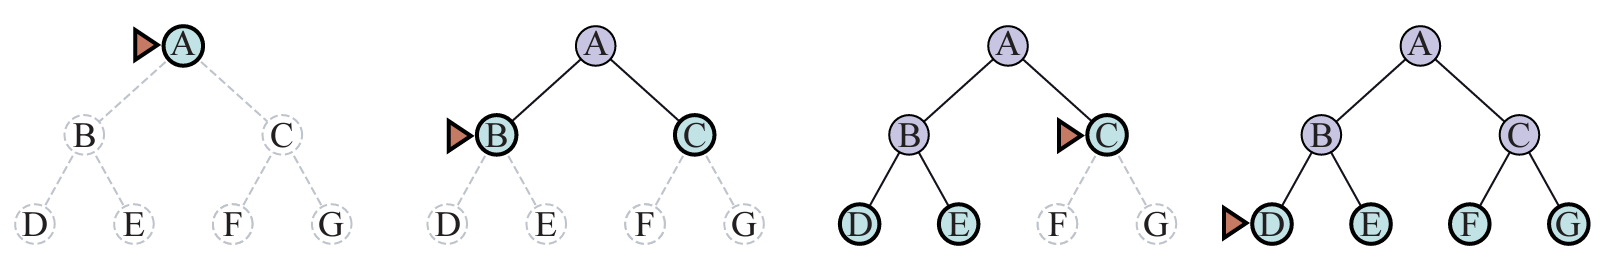
\includegraphics[scale=0.45]{./img/BFS}
\end{figure}

\end{frame} 
%%%%%%%%%%%%%%%%%%%%%%%%%%%%%%%%

%%%%%%%%%%%%%%%%%%%%%%%%%%%%%%%%
\begin{frame} \frametitle{Amplitud (Breadth)} \footnotesize
\begin{itemize}
\item En términos de tiempo y espacio nos ponemos en el caso donde cada estado tiene b sucesores.

\item La raíz de cada árbol genera b nodos, cada uno de ellos generan b nodos más, en un total de $b^2$ en el segundo nivel, y $b^3$ en el tercer nivel $\ldots$

\item Suponemos que la solución está en un nivel d, entonces el número de nodos generados es:

\begin{center}
$1+b+b^2+b^3+ \ldots +b^d =O(b^d)$    
\end{center}

\item Todos los nodos se mantienen en memoria, por lo que la complejidad en tiempo y espacio son $O(b^d)$.

\item Un ejemplo en el mundo real podría ser un factor b = 10. Si tenemos la capacidad de procesar 1 millón de nodos por segundo y cada nodo ocupa un 1Kbyte. En una profundidad de d=10  ($O(b^d) = O(10^{10}) = 10,000,000,000 $) el procesamiento de los nodos llevaría más de 3 horas y necesitaria 10 terabytes de memoria.

\item \textbf{Los requisitos de memoria son un mayor problema que el tiempo de ejecución.}

\end{itemize}


\end{frame} 
%%%%%%%%%%%%%%%%%%%%%%%%%%%%%%%%

%%%%%%%%%%%%%%%%%%%%%%%%%%%%%%%%
\begin{frame} \frametitle{Amplitud (Breadth)} \footnotesize


\begin{figure}
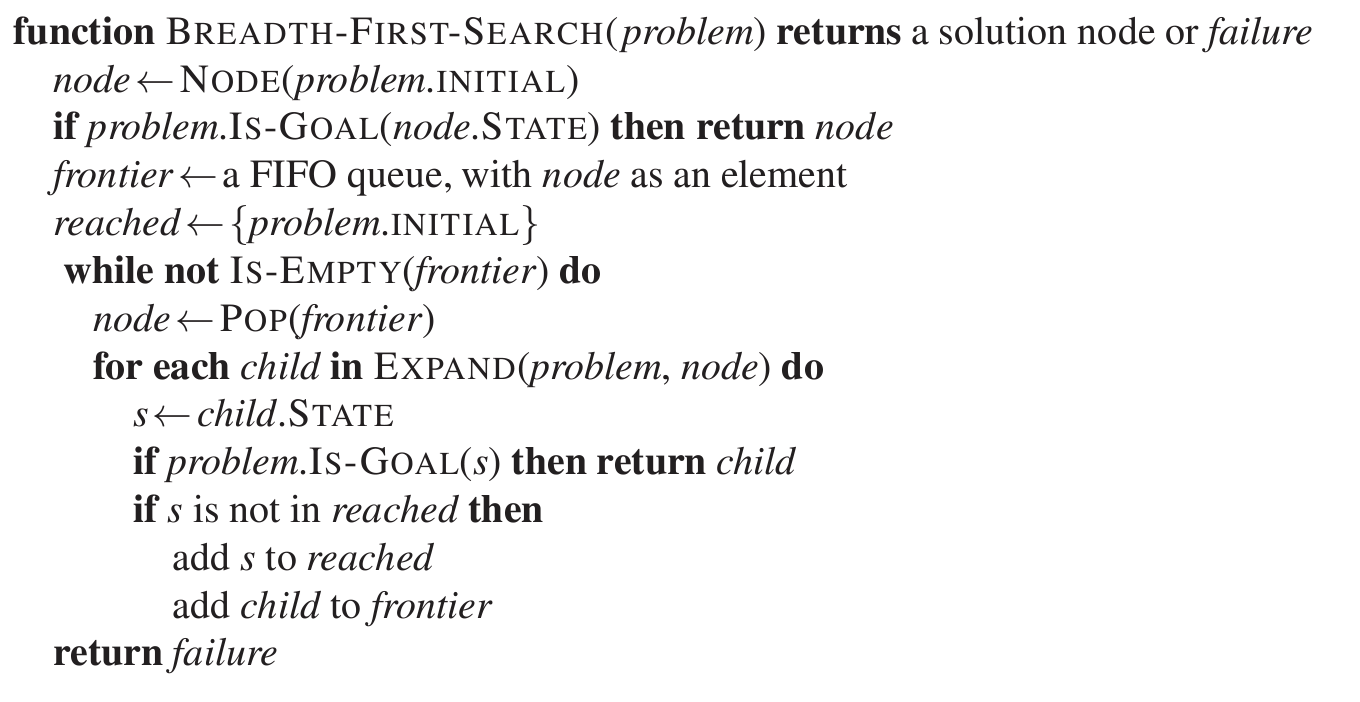
\includegraphics[scale=0.45]{./img/BFS_algorithm}
\end{figure}

\end{frame} 

%%%%%%%%%%%%%%%%%%%%%%%%%%%%%%%%
\begin{frame} [fragile ]\frametitle{Amplitud  en Python } \footnotesize
\begin{minted}[fontsize=\tiny]{python}
def breadth_first_search(problem):
    longitud_frontera = 0 
    node = Node(problem.initial_state)
    if problem.is_goal(node.state):
        return node
    frontier = deque([node])
    reached = {tuple(problem.initial_state)}
    while frontier:
        node = frontier.popleft()
        print (node)
        for child_state in problem.expand(node.state):
            print (child_state)
            if tuple(child_state) not in reached:
                child_node = Node(child_state, node)
                if problem.is_goal(child_state):
                    print (f"SOL={child_state}")
                    print (f"max frontier longitud = {longitud_frontera}")
                    return child_node
                reached.add(tuple(child_state))
                frontier.append(child_node)
                if (longitud_frontera < len(frontier)):
                    longitud_frontera = len(frontier)
    return "failure"
\end{minted}

\end{frame} 
%%%%%%%%%%%%%%%%%%%%%%%%%%%%%%%%
\begin{frame} [fragile ]\frametitle{Amplitud  en Python } \footnotesize
\begin{minted}[fontsize=\small]{python}
class Node:
    def __init__(self, state, parent=None):
        self.state = state
        self.parent = parent
    def __str__(self):
        return f"Node(state={self.state}, parent={self.parent})"    

\end{minted}

\end{frame} 

        
%%%%%%%%%%%%%%%%%%%%%%%%%%%%%%%%
\begin{frame} \frametitle{Ejemplo Grafo - Amplitud} \scriptsize



\begin{columns}
\begin{column}{0.6\textwidth}

 \begin{center}
     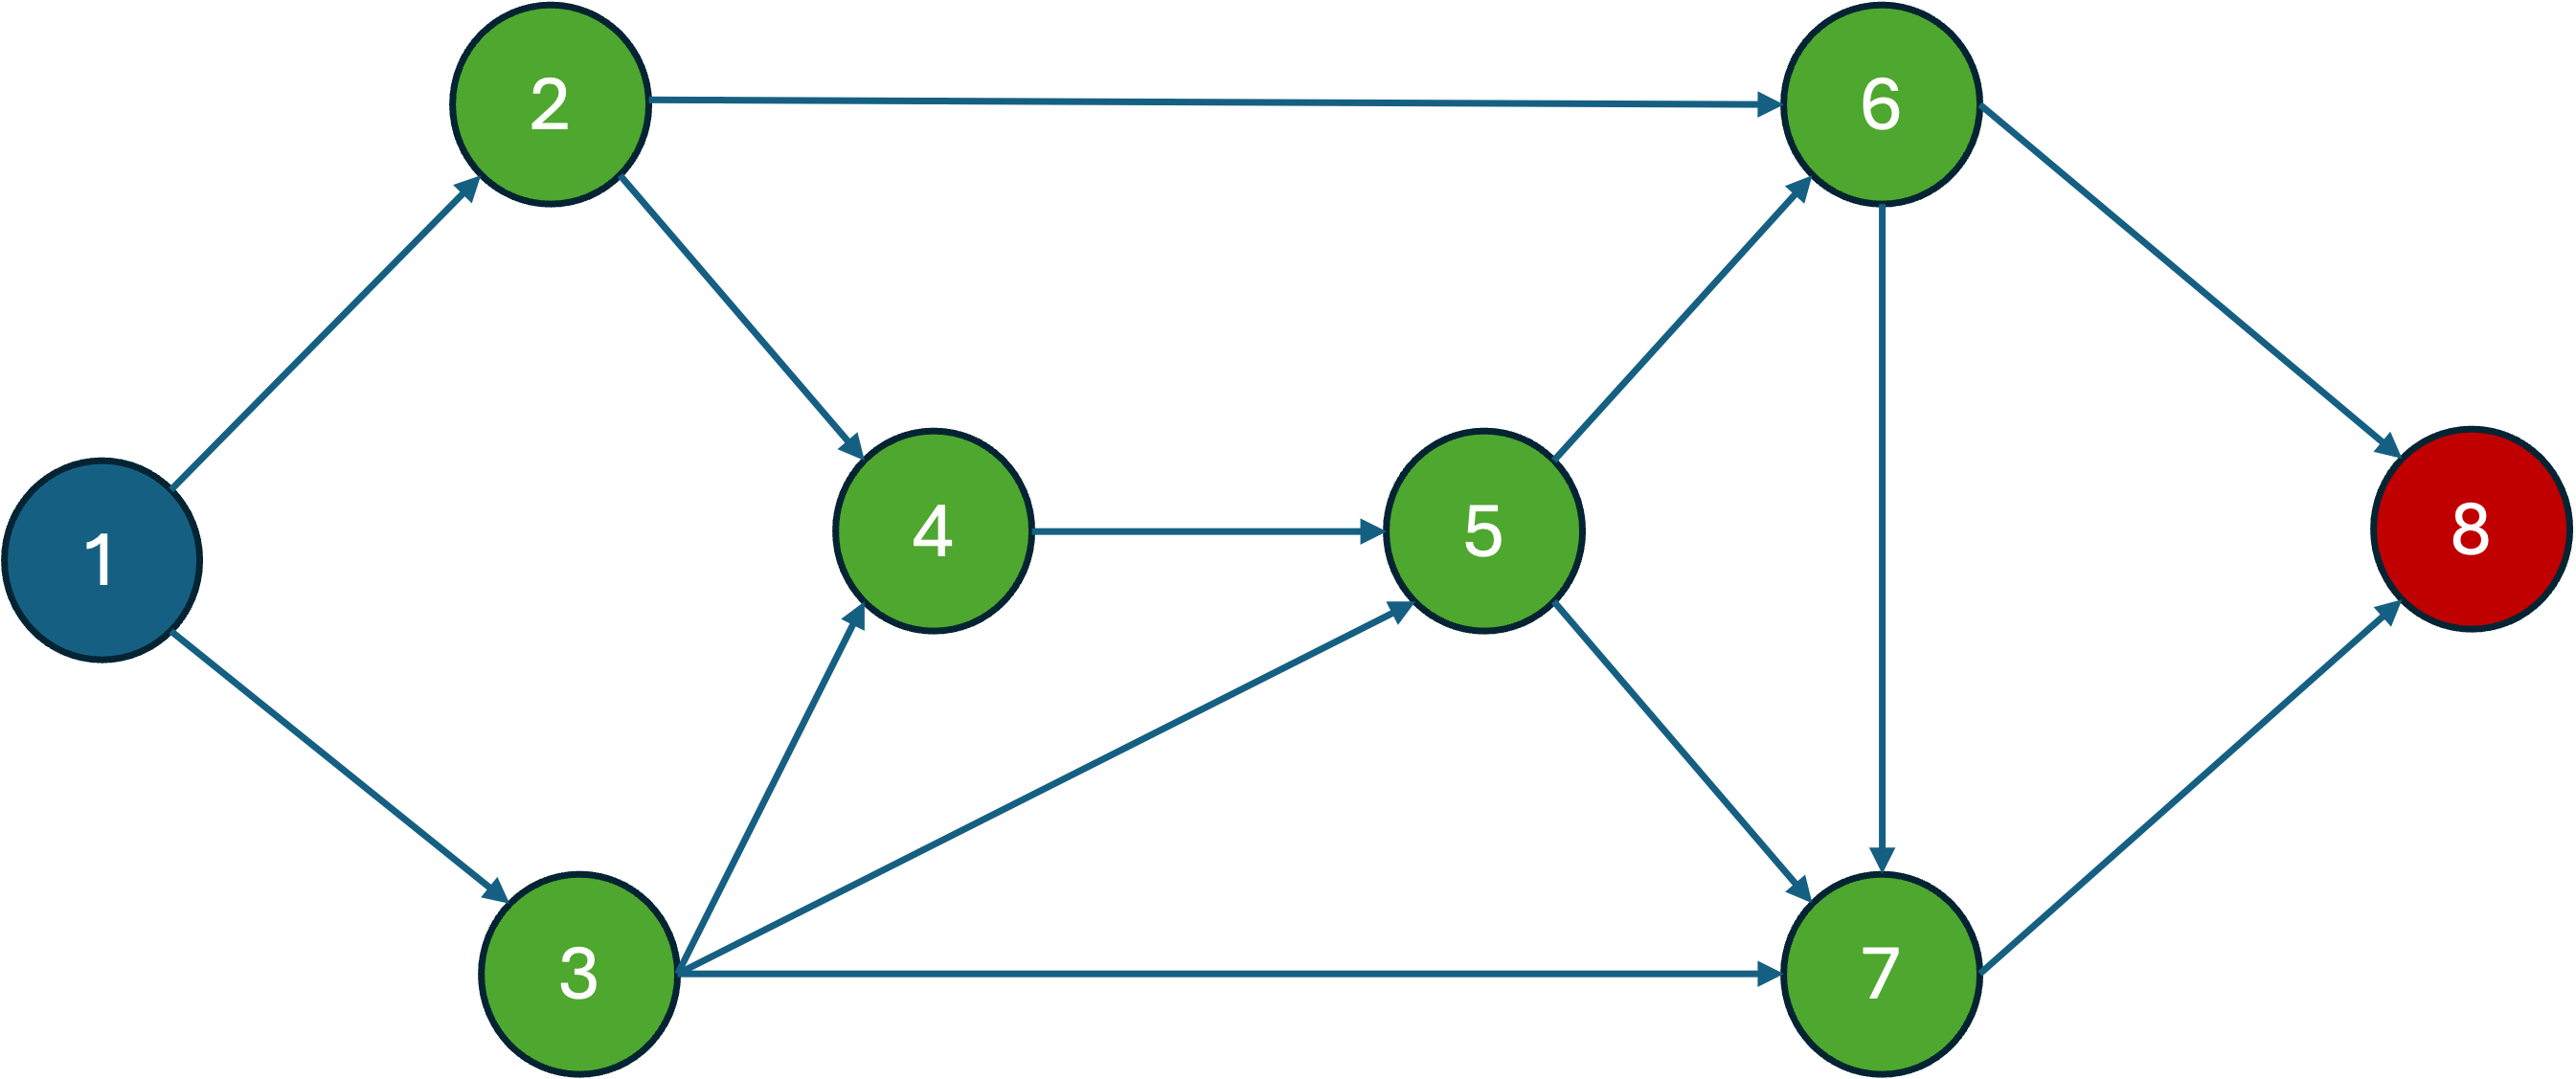
\includegraphics[width=0.6\textwidth]{img/GrafoEjemplo1}
     \end{center}
     
\begin{itemize}\scriptsize
    \item Nodo 1 -  Expando nodo 1 - (2,3) Frontera: 2, 3\\
    \item Nodo 2 -  Expando nodo 2 - (4,6) Frontera: 3, 4, 6\\
    \item Nodo 3 - Expando nodo 3 - (4,5,7) Frontera: 4, 6, 5, 7 (4 Repetido)\\
    \item Nodo 4 - Expando nodo 4 - (5) Frontera: 6, 5, 7 (5 Repetido)\\
    \item Nodo 6 - Expando nodo 6 - (7,8) Frontera: 5, 7, 8 (7 Repetido)\\
    \item 8 SOL\\
\end{itemize}


\end{column}
\begin{column}{0.4\textwidth}  
    \begin{center}
     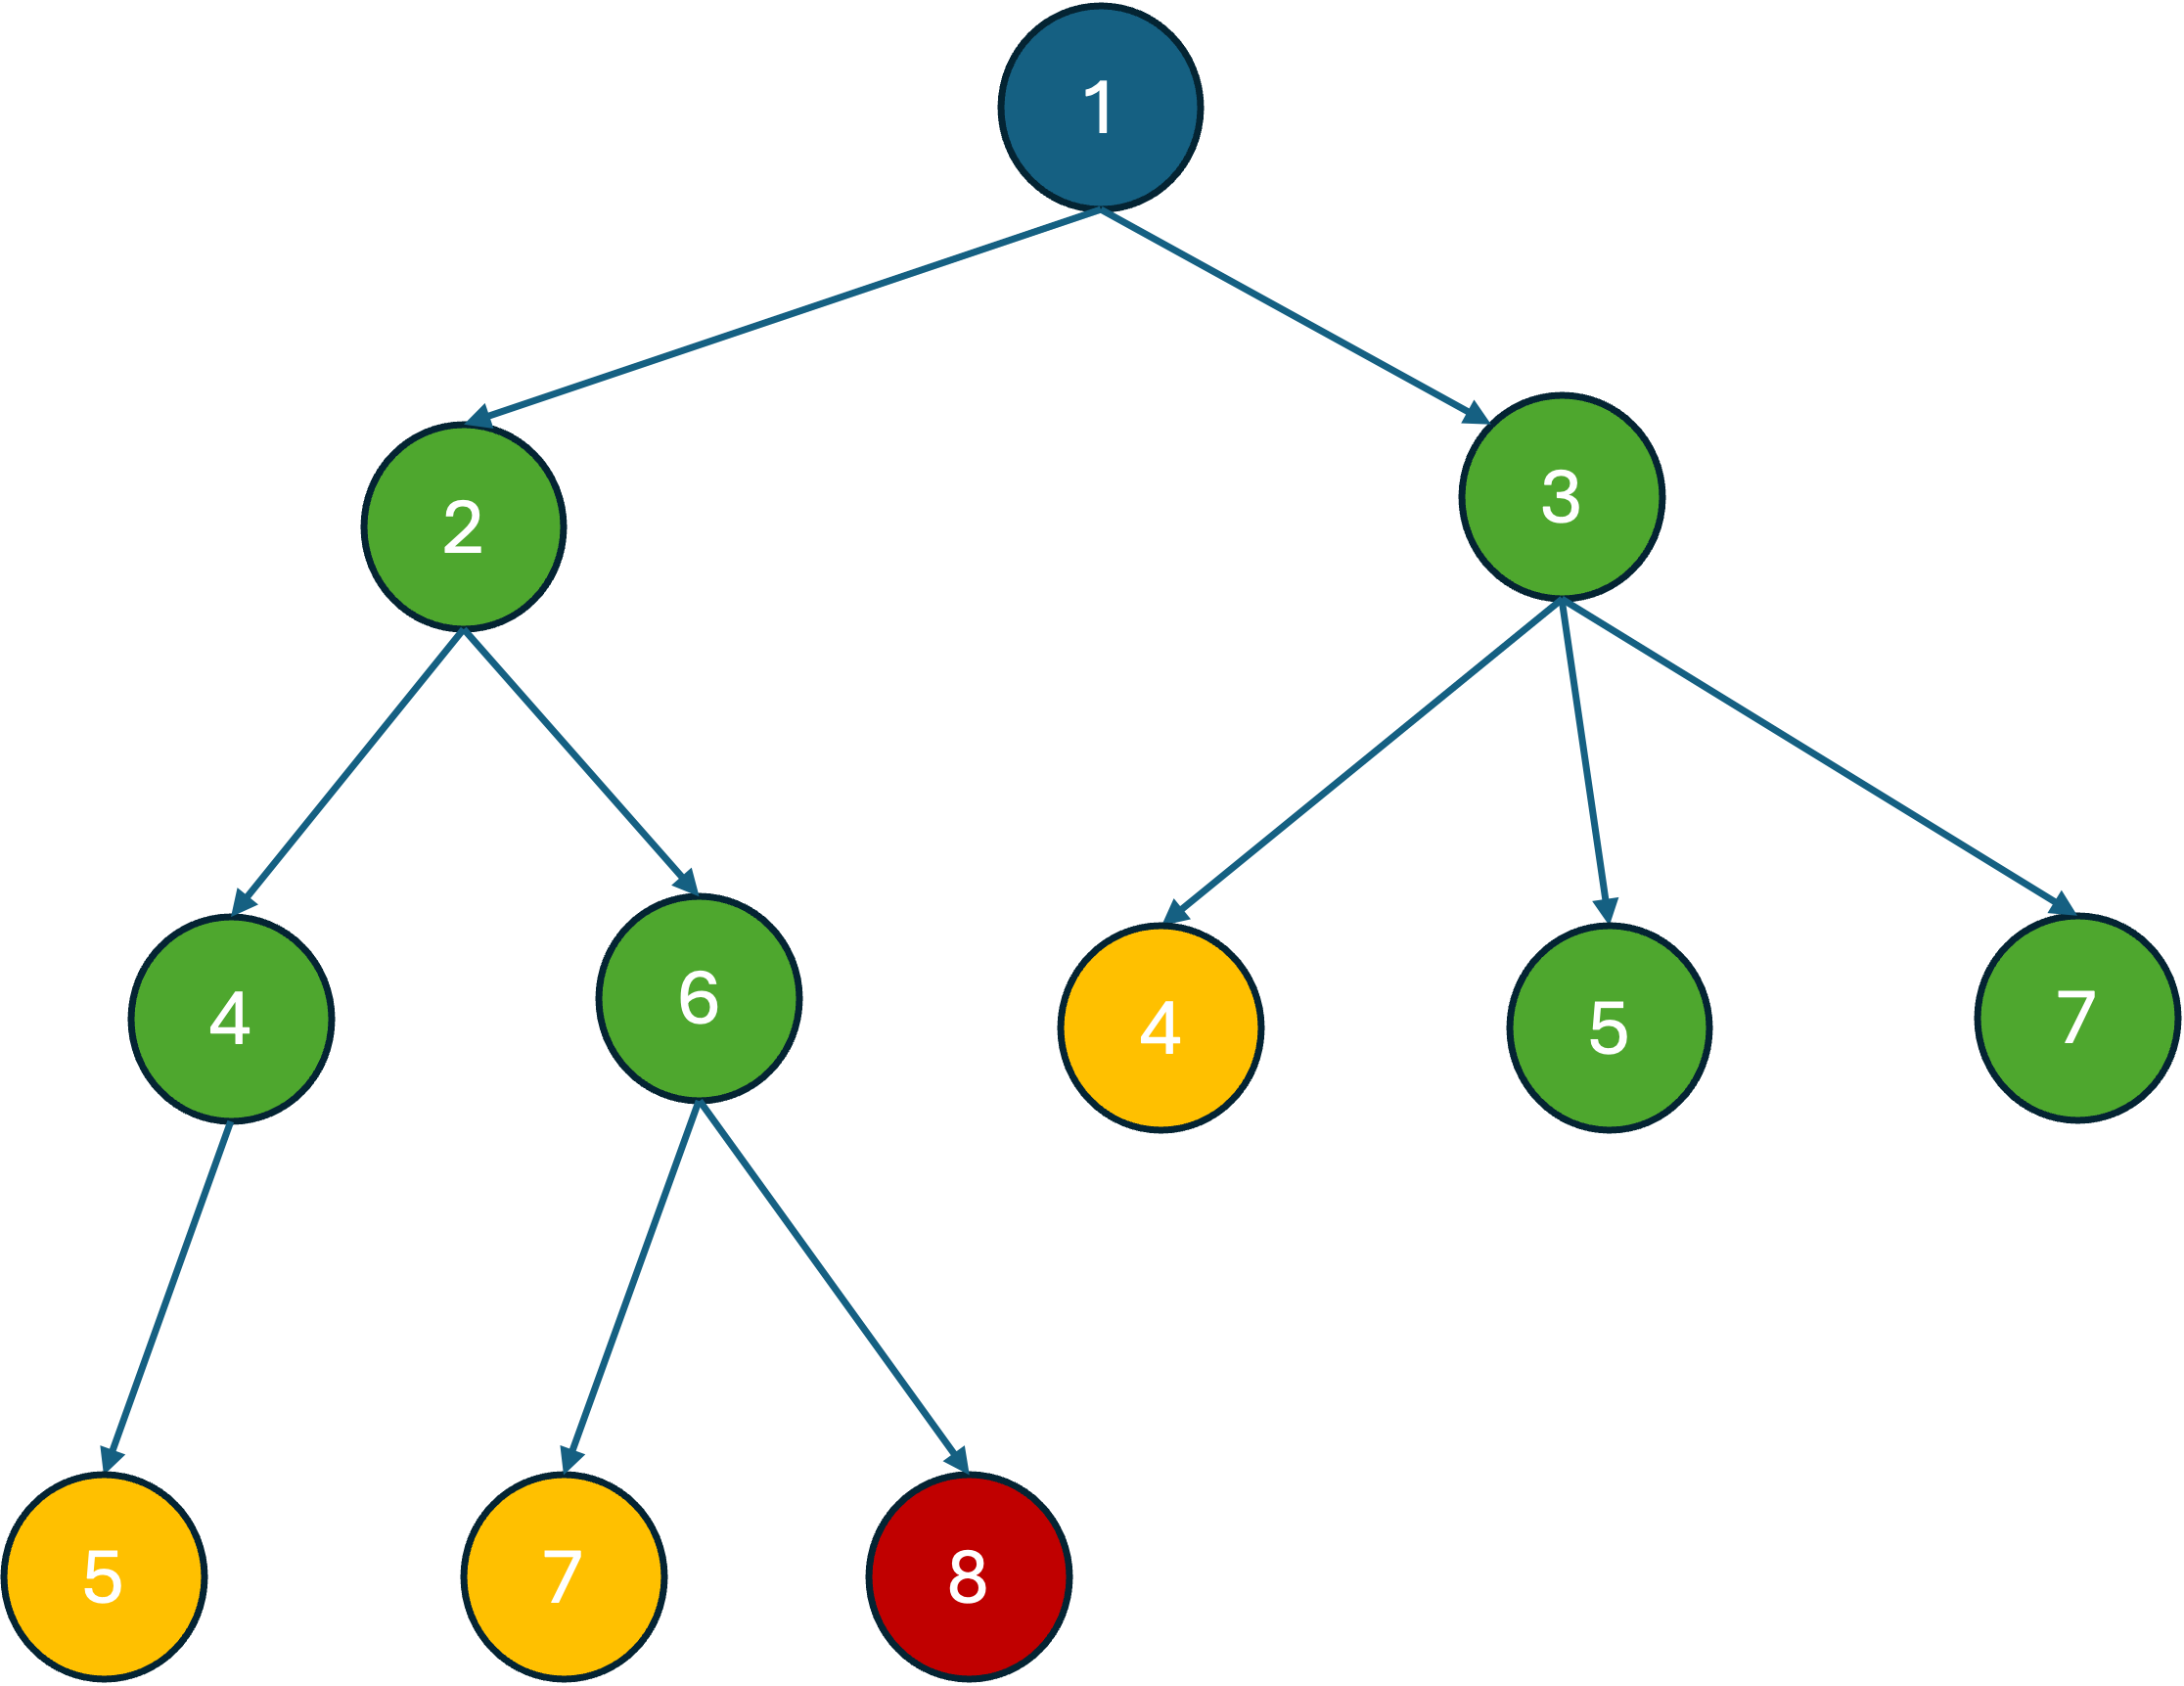
\includegraphics[width=\textwidth]{img/ArbolAmplitud.png}
     \end{center}
\end{column}
\end{columns}


\end{frame} 
%%%%%%%%%%%%%%%%%%%%%%%%%%%%%%%%

%%%%%%%%%%%%%%%%%%%%%%%%%%%%%%%%
\begin{frame} [fragile ]\frametitle{Problema Grafo  en Python } \footnotesize
\begin{minted}[fontsize=\tiny]{python}
class ProblemGrafo:
    def __init__(self, initial_state, goal_state):
        self.initial_state = initial_state
        self.goal_state = goal_state

    def is_goal(self, state):
        return state == self.goal_state

    def expand(self, state):
        # Define cómo expandir un estado para obtener los posibles estados hijos
        sucesores = { 
            '1': ['2', '3'],
            '2': ['4', '6'],
            '3': ['4', '5', '7'],
            '4': ['5'],
            '5': ['6', '7'],
            '6': ['7', '8'],
            '7': ['8']
        }
        return sucesores.get(state, [])  # Devuelve los vecinos del estado o una lista vacía si el estado no tiene vecinos

\end{minted}

\end{frame} 

%%%%%%%%%%%%%%%%%%%%%%%%%%%%%%%%
\begin{frame} [fragile ]\frametitle{Problema Grafo  en Python } \small
\begin{minted}[fontsize=\small]{python}
initial_state = '1'
goal_state = '8'
problem = ProblemGrafo(initial_state, goal_state)
solution_node = breadth_first_search(problem)

\end{minted}

\end{frame} 

%%%%%%%%%%%%%%%%%%%%%%%%%%%%%%%%
\begin{frame} \frametitle{Puzzle 8} \scriptsize

Es un rompecabezas de fichas deslizantes. Una serie de fichas  se colocan en una cuadrícula con un espacio en blanco para que el resto de las fichas puedan deslizarse en el espacio en blanco.\\

La formulación estándar del puzzle 8 es la siguiente: 

\begin{itemize}
    \item \textbf{Estados}: Una descripción de estado especifica la ubicación de cada una de las fichas. 
    \begin{itemize}\scriptsize
    \item Estado inicial: Cualquier estado puede ser designado como estado inicial.
    \end{itemize}
    \item \textbf{Acciones}: Mientras que en el mundo físico es una ficha la que se desliza, la forma más sencilla de describir una acción es pensar que el espacio en blanco se mueve hacia la izquierda, derecha, arriba o abajo. Si el espacio en blanco está en un borde o una esquina, no todas las acciones serán aplicables.
    \item \textbf{Estado objetivo}: Aunque cualquier estado podría ser el objetivo, normalmente especificamos un estado con los números en orden.
    \item \textbf{Modelo de transición}: Asigna un estado y una acción a un estado resultante;
    \item \textbf{Coste de la acción}: Cada acción cuesta 1.
\end{itemize}

\begin{figure}

\includegraphics[scale=0.25]{./img/Puzzle8}
\end{figure}

\end{frame} 
%%%%%%%%%%%%%%%%%%%%%%%%%%%%%%%%
\begin{frame} [fragile ]\frametitle{Puzzle 8  en Python } \footnotesize
\begin{minted}[fontsize=\tiny]{python}
class Puzzle8Problem:
    def __init__(self, initial_state, goal_state):
        self.initial_state = initial_state
        self.goal_state = goal_state

    def is_goal(self, state):
        return state == self.goal_state

    def expand(self, state):
        children = []
        zero_index = (state.index(0) // 3, state.index(0) % 3)
        moves = [(1, 0), (-1, 0), (0, 1), (0, -1)]  # Movimientos: arriba, abajo, izquierda, derecha
        for move in moves:
            new_index = (zero_index[0] + move[0], zero_index[1] + move[1])
            if 0 <= new_index[0] < 3 and 0 <= new_index[1] < 3:  # Verificar límites
                new_state = list(state)
                new_state[zero_index[0] * 3 + zero_index[1]], new_state[new_index[0] * 3 + new_index[1]] = \
                    new_state[new_index[0] * 3 + new_index[1]], new_state[zero_index[0] * 3 + zero_index[1]]
                children.append(new_state)
        return children

\end{minted}

\end{frame} 

%%%%%%%%%%%%%%%%%%%%%%%%%%%%%%%%
\begin{frame} [fragile ]\frametitle{Ejecución Puzzle 8  en Python } \footnotesize
\begin{minted}[fontsize=\footnotesize]{python}
initial_state = [1, 2 , 0, 3, 4, 5, 6, 7, 8]
goal_state = [0, 1, 2, 3, 4, 5, 6, 7, 8]
problem = Puzzle8Problem(initial_state, goal_state)
solution_node = breadth_first_search(problem)

\end{minted}

\end{frame} 

%%%%%%%%%%%%%%%%%%%%%%%%%%%%%%%%
\begin{frame} [fragile ]\frametitle{Imprimir Solución Problema Puzzle 8  en Python } \footnotesize
\begin{minted}[fontsize=\footnotesize]{python}
def print_solution (solution_node):
    # Reconstruir la ruta hacia la solución
    if solution_node != "failure":
        path = []
        while solution_node:
            path.append(solution_node.state)
            solution_node = solution_node.parent
        path.reverse()
        print("\n\nSolución encontrada:\n")
        for state in path:
            #imprimirTablero(state)
            print(state)
    else:
        print("No se encontró solución.")

\end{minted}

\end{frame} 

%%%%%%%%%%%%%%%%%%%%%%%%%%%%%%%%
\begin{frame} [fragile ]\frametitle{Puzzle 8 } \footnotesize
Estado inicial "fácil"
\begin{minted}[fontsize=\tiny]{python}

initial_state = [1, 2 , 0, 3, 4, 5, 6, 7, 8]
goal_state = [0, 1, 2, 3, 4, 5, 6, 7, 8]

Node(state=[1, 2, 0, 3, 4, 5, 6, 7, 8], parent=None)
[1, 2, 5, 3, 4, 0, 6, 7, 8]
[1, 0, 2, 3, 4, 5, 6, 7, 8]
Node(state=[1, 2, 5, 3, 4, 0, 6, 7, 8], parent=Node(state=[1, 2, 0, 3, 4, 5, 6, 7, 8], parent=None))
[1, 2, 5, 3, 4, 8, 6, 7, 0]
[1, 2, 0, 3, 4, 5, 6, 7, 8]
[1, 2, 5, 3, 0, 4, 6, 7, 8]
Node(state=[1, 0, 2, 3, 4, 5, 6, 7, 8], parent=Node(state=[1, 2, 0, 3, 4, 5, 6, 7, 8], parent=None))
[1, 4, 2, 3, 0, 5, 6, 7, 8]
[1, 2, 0, 3, 4, 5, 6, 7, 8]
[0, 1, 2, 3, 4, 5, 6, 7, 8]
SOL=[0, 1, 2, 3, 4, 5, 6, 7, 8]

max frontier longitud = 3
\end{minted}

\end{frame} 
%%%%%%%%%%%%%%%%%%%%%%%%%%%%%%%%
\begin{frame} [fragile ]\frametitle{Puzzle 8} \footnotesize
\textbf{Estado inicial "fácil"}\\
\hspace{2cm}


[1, 2, 0, 3, 4, 5, 6, 7, 8] \textbf{IZQ} \newline
[1, 0, 2, 3, 4, 5, 6, 7, 8] \textbf{IZQ} \newline
[0, 1, 2, 3, 4, 5, 6, 7, 8]\newline

\end{frame} 

%%%%%%%%%%%%%%%%%%%%%%%%%%%%%%%%
\begin{frame} [fragile ]\frametitle{Puzzle 8} \footnotesize
\textbf{Estado inicial "fácil"}
\begin{figure}
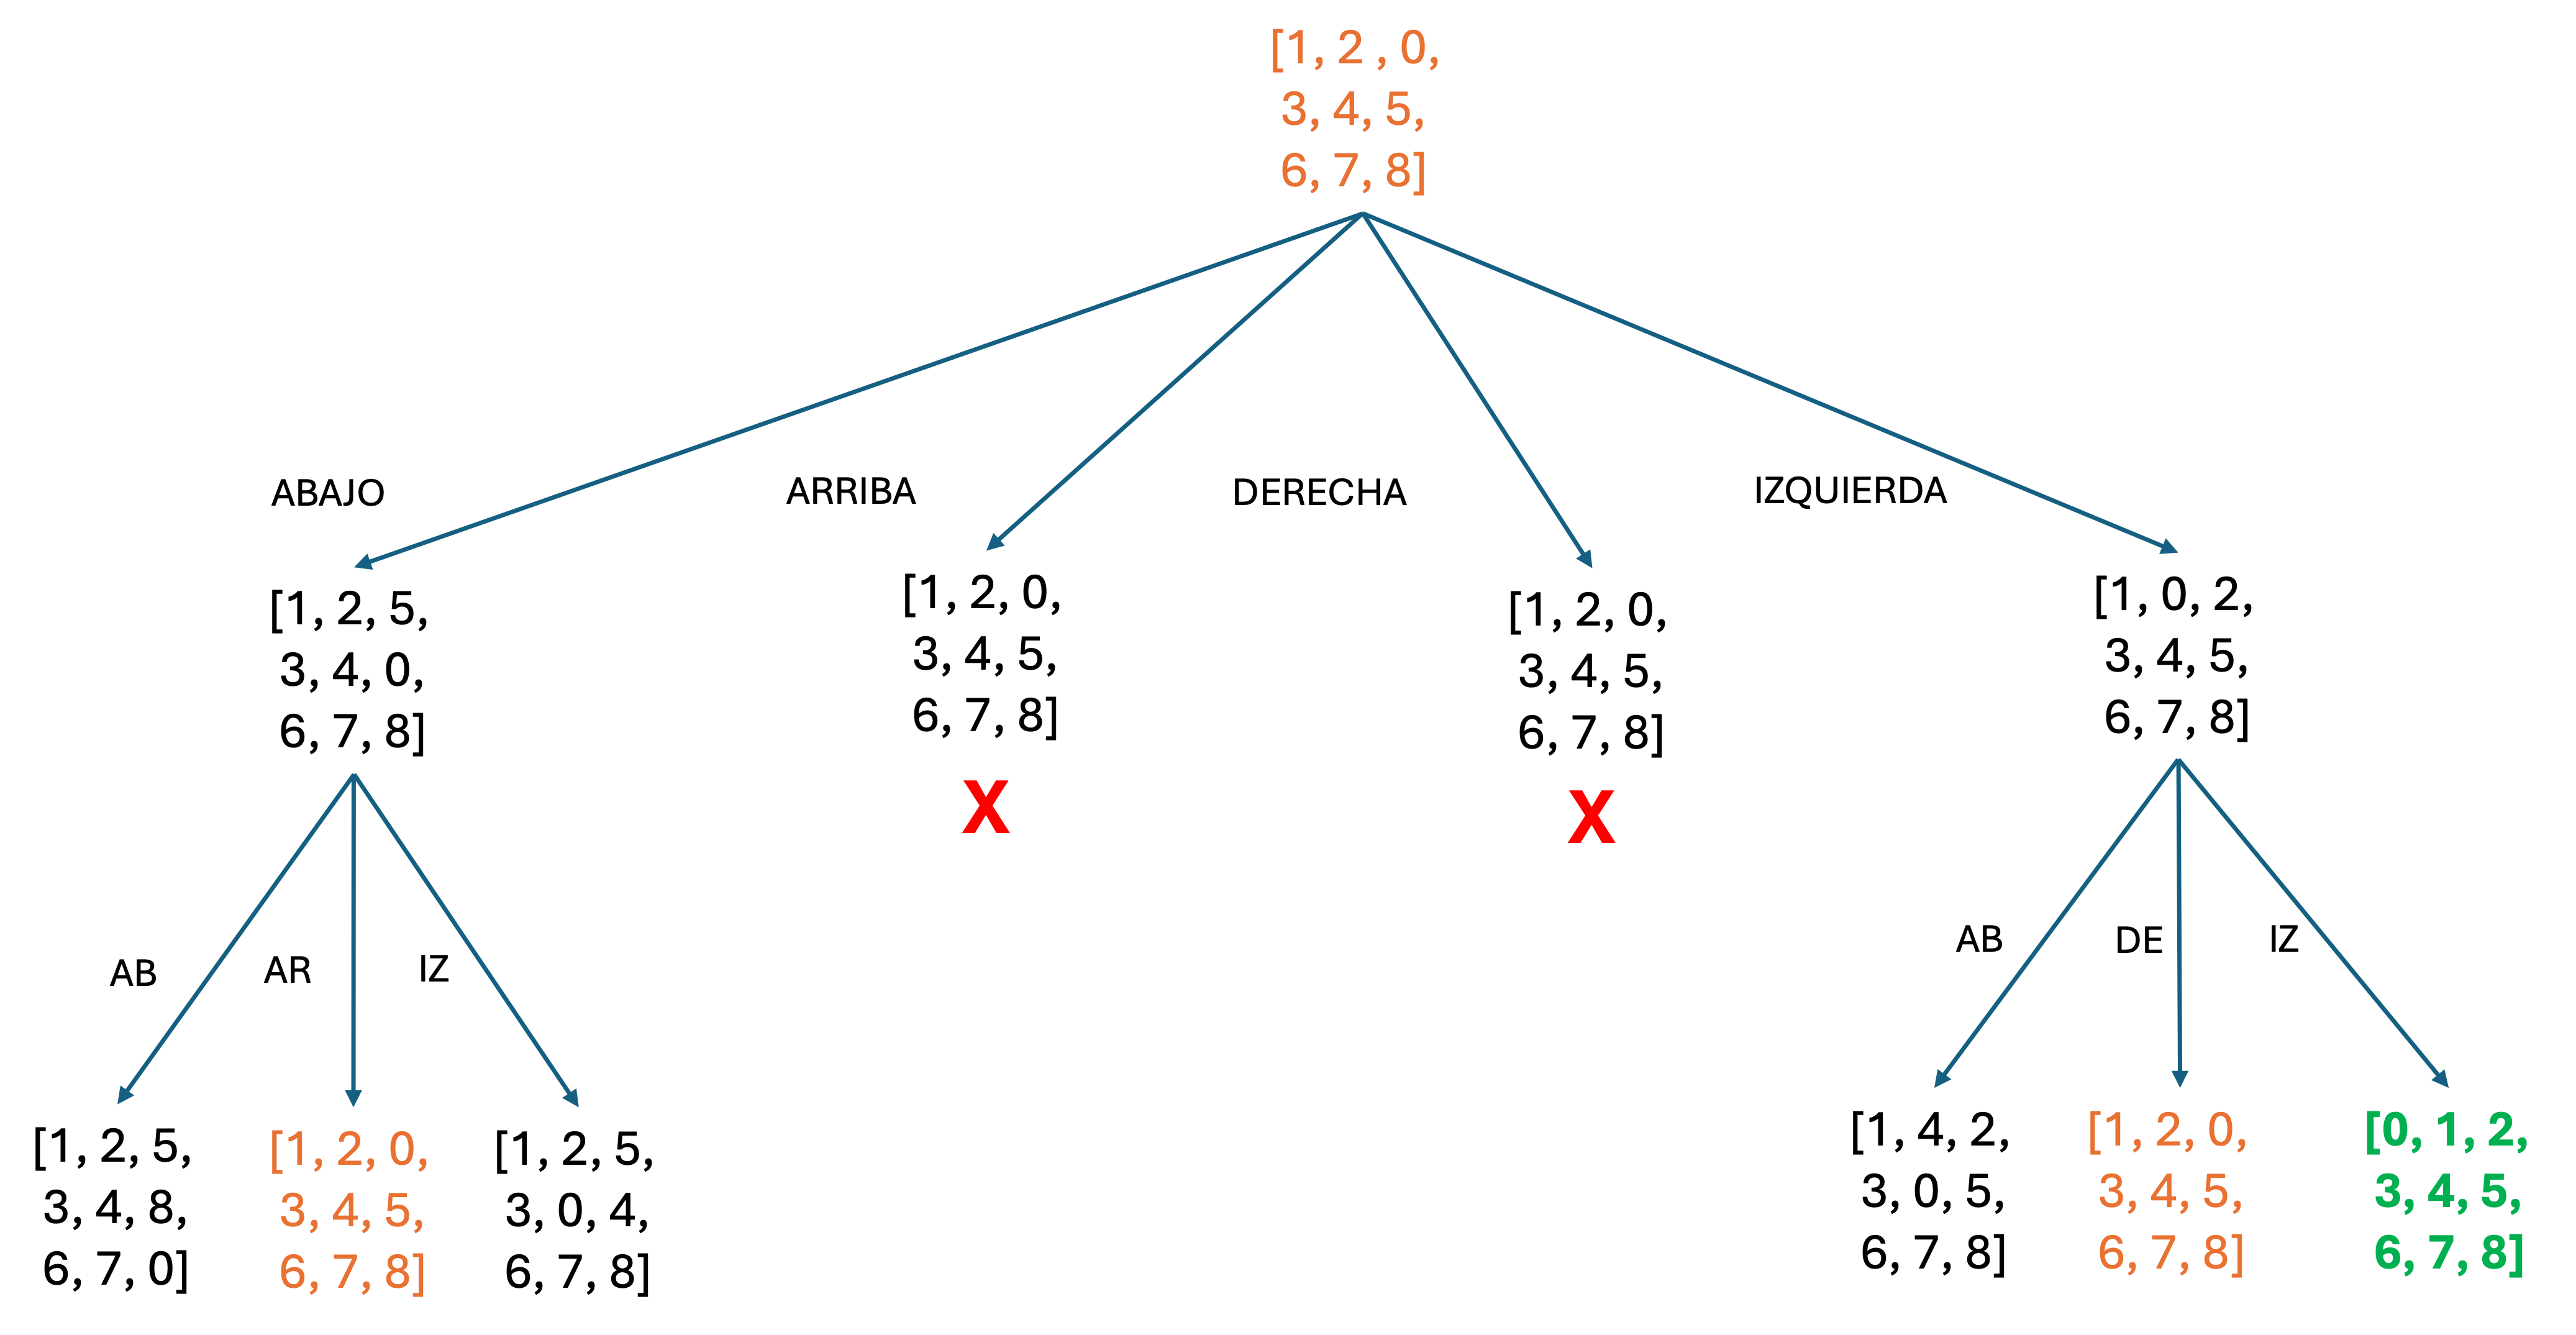
\includegraphics[scale=0.35]{./img/PuzzleFacilarbol}
\end{figure}
\end{frame} 

%%%%%%%%%%%%%%%%%%%%%%%%%%%%%%%%
\begin{frame} [fragile ]\frametitle{Puzzle 8} \footnotesize
\textbf{Estado inicial "no tan fácil"}
\begin{minted}[fontsize=\tiny]{python}

initial_state = [1, 2, 3, 0, 4, 6, 7, 5, 8]
goal_state = [0, 1, 2, 3, 4, 5, 6, 7, 8]

Node(state=[1, 2, 3, 0, 4, 6, 7, 5, 8], parent=None)
[1, 2, 3, 7, 4, 6, 0, 5, 8]
[0, 2, 3, 1, 4, 6, 7, 5, 8]
[1, 2, 3, 4, 0, 6, 7, 5, 8]
...
...
...
Node(state=[3, 0, 2, 4, 1, 5, 6, 7, 8], parent=Node(state=[3, 1, 2, 4, 0, 5, 6, 7, 8], parent=Node(state=[3, 1, 2, 4, 5, 0, 6, 7, 8], parent=Node(state=[3, 1, 0, 4, 5, 2, 6, 7, 8], parent=Node(state=[3, 0, 1, 4, 5, 2, 6, 7, 8], parent=Node(state=[0, 3, 1, 4, 5, 2, 6, 7, 8], parent=Node(state=[4, 3, 1, 0, 5, 2, 6, 7, 8], parent=Node(state=[4, 3, 1, 6, 5, 2, 0, 7, 8], parent=Node(state=[4, 3, 1, 6, 5, 2, 7, 0, 8], parent=Node(state=[4, 3, 1, 6, 0, 2, 7, 5, 8], parent=Node(state=[4, 0, 1, 6, 3, 2, 7, 5, 8], parent=Node(state=[4, 1, 0, 6, 3, 2, 7, 5, 8], parent=Node(state=[4, 1, 2, 6, 3, 0, 7, 5, 8], parent=Node(state=[4, 1, 2, 6, 0, 3, 7, 5, 8], parent=Node(state=[4, 1, 2, 0, 6, 3, 7, 5, 8], parent=Node(state=[0, 1, 2, 4, 6, 3, 7, 5, 8], parent=Node(state=[1, 0, 2, 4, 6, 3, 7, 5, 8], parent=Node(state=[1, 2, 0, 4, 6, 3, 7, 5, 8], parent=Node(state=[1, 2, 3, 4, 6, 0, 7, 5, 8], parent=Node(state=[1, 2, 3, 4, 0, 6, 7, 5, 8], parent=Node(state=[1, 2, 3, 0, 4, 6, 7, 5, 8], parent=None)))))))))))))))))))))
[3, 1, 2, 4, 0, 5, 6, 7, 8]
[3, 2, 0, 4, 1, 5, 6, 7, 8]
[0, 3, 2, 4, 1, 5, 6, 7, 8]
Node(state=[3, 1, 2, 0, 4, 5, 6, 7, 8], parent=Node(state=[3, 1, 2, 4, 0, 5, 6, 7, 8], parent=Node(state=[3, 1, 2, 4, 5, 0, 6, 7, 8], parent=Node(state=[3, 1, 0, 4, 5, 2, 6, 7, 8], parent=Node(state=[3, 0, 1, 4, 5, 2, 6, 7, 8], parent=Node(state=[0, 3, 1, 4, 5, 2, 6, 7, 8], parent=Node(state=[4, 3, 1, 0, 5, 2, 6, 7, 8], parent=Node(state=[4, 3, 1, 6, 5, 2, 0, 7, 8], parent=Node(state=[4, 3, 1, 6, 5, 2, 7, 0, 8], parent=Node(state=[4, 3, 1, 6, 0, 2, 7, 5, 8], parent=Node(state=[4, 0, 1, 6, 3, 2, 7, 5, 8], parent=Node(state=[4, 1, 0, 6, 3, 2, 7, 5, 8], parent=Node(state=[4, 1, 2, 6, 3, 0, 7, 5, 8], parent=Node(state=[4, 1, 2, 6, 0, 3, 7, 5, 8], parent=Node(state=[4, 1, 2, 0, 6, 3, 7, 5, 8], parent=Node(state=[0, 1, 2, 4, 6, 3, 7, 5, 8], parent=Node(state=[1, 0, 2, 4, 6, 3, 7, 5, 8], parent=Node(state=[1, 2, 0, 4, 6, 3, 7, 5, 8], parent=Node(state=[1, 2, 3, 4, 6, 0, 7, 5, 8], parent=Node(state=[1, 2, 3, 4, 0, 6, 7, 5, 8], parent=Node(state=[1, 2, 3, 0, 4, 6, 7, 5, 8], parent=None)))))))))))))))))))))
[3, 1, 2, 6, 4, 5, 0, 7, 8]
[0, 1, 2, 3, 4, 5, 6, 7, 8]
SOL=[0, 1, 2, 3, 4, 5, 6, 7, 8]

max frontier longitud = 21703
\end{minted}

\end{frame} 

%%%%%%%%%%%%%%%%%%%%%%%%%%%%%%%%
\begin{frame} [fragile ]\frametitle{Puzzle 8} \footnotesize
\textbf{Estado inicial "no tan fácil"}\\
\hspace{2cm}

[1, 2, 3, 0, 4, 6, 7, 5, 8] [1, 2, 3, 4, 0, 6, 7, 5, 8]
[1, 2, 3, 4, 6, 0, 7, 5, 8] 
[1, 2, 0, 4, 6, 3, 7, 5, 8]
[1, 0, 2, 4, 6, 3, 7, 5, 8]\newline
[0, 1, 2, 4, 6, 3, 7, 5, 8] [4, 1, 2, 0, 6, 3, 7, 5, 8]
[4, 1, 2, 6, 0, 3, 7, 5, 8]
[4, 1, 2, 6, 3, 0, 7, 5, 8]
[4, 1, 0, 6, 3, 2, 7, 5, 8]\newline
[4, 0, 1, 6, 3, 2, 7, 5, 8]
[4, 3, 1, 6, 0, 2, 7, 5, 8]
[4, 3, 1, 6, 5, 2, 7, 0, 8]
[4, 3, 1, 6, 5, 2, 0, 7, 8]
[4, 3, 1, 0, 5, 2, 6, 7, 8]\newline
[0, 3, 1, 4, 5, 2, 6, 7, 8]
[3, 0, 1, 4, 5, 2, 6, 7, 8]
[3, 1, 0, 4, 5, 2, 6, 7, 8]
[3, 1, 2, 4, 5, 0, 6, 7, 8]
[3, 1, 2, 4, 0, 5, 6, 7, 8]\newline
[3, 1, 2, 0, 4, 5, 6, 7, 8]
[0, 1, 2, 3, 4, 5, 6, 7, 8]


\end{frame} 

%%%%%%%%%%%%%%%%%%%%%%%%%%%%%%%%
%%%%%%%%%%%%%%%%%%%%%%%%%%%%%%%%
%%%%%%%%%%%%%%%%%%%%%%%%%%%%%%%%
\subsection{Algoritmo de Dijkstra o búsqueda de coste uniforme }
\begin{chapter}[images/etsiinformatica4.png]{uicblue}{Algoritmo de Dijkstra o búsqueda de coste uniforme }
\end{chapter}



%%%%%%%%%%%%%%%%%%%%%%%%%%%%%%%%
\begin{frame} \frametitle{Algoritmo de Dijkstra o búsqueda de coste uniforme } \small
\begin{itemize}

\item Cuando las acciones tienen diferentes costes, una opción obvia es utilizar la búsqueda del mejor primero (veremos en el próximo tema), en la que la función de evaluación es el coste del camino desde la raíz hasta el nodo actual.

\item La idea es que, mientras que la búsqueda de amplitud primero se extiende en base a una profundidad uniforme -primero profundidad 1, luego profundidad 2, y así sucesivamente-, la búsqueda de coste uniforme lo hace basándose en el coste de la trayectoria.

\item Expandimos el nodo n con el coste del camino más pequeño.
	\begin{itemize}
		\item Si son todos iguales es idéntico a la búsqueda en amplitud.
	\end{itemize}
	
\item No se preocupa por el \textbf{número de pasos} que tiene un camino, pero sí por su \textbf{coste total}. 
	
	
\end{itemize}

\end{frame} 

%%%%%%%%%%%%%%%%%%%%%%%%%%%%%%%%
\begin{frame} \frametitle{Algoritmo de Dijkstra o búsqueda de coste uniforme } \footnotesize

\begin{columns}
\begin{column}{0.6\textwidth}

\textbf{El problema es cómo ir de  Sibiu a Bucharest}.\\ 

\begin{itemize}\footnotesize
    \item Los sucesores de Sibiu son Rimnicu Vilcea (80) y Fagaras (99).\\
    \item El siguiente nodo expandido es el nodo con menor coste, Rimnicu Vilcea, añadiendo Pitesti con coste total 80+97=177. 
    \item En este punto tenemos disponible Fagaras (99) y Pitesti(177) con lo cual elegimos Fagaras y añadimos Bucharest con coste 211, que hacen un total de 310.
    \item Bucharest es el objetivo, pero no se verifica el objetivo hasta que se expande un nodo, por lo que hay dos nodos abiertos Bucharest con 310 y  Pitesti con 177, por tanto expandimos y obtenemos un coste de 278 hasta Bucharest.
\end{itemize}

\end{column}
\begin{column}{0.4\textwidth}  
    \begin{center}
     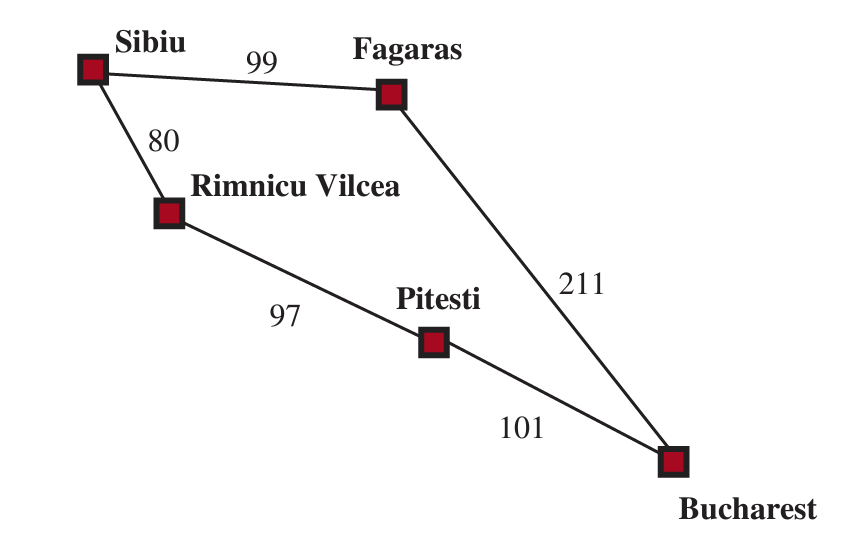
\includegraphics[width=\textwidth]{img/EjemploDijkstra.png}
     \end{center}
\end{column}
\end{columns}


\end{frame} 


%%%%%%%%%%%%%%%%%%%%%%%%%%%%%%%%
\begin{frame} [fragile ]\frametitle{Dijkstra  en Python } \footnotesize
\begin{minted}[fontsize=\footnotesize]{python}

class NodeCost:
    def __init__(self, state, cost, parent=None):
        self.state = state
        self.cost = cost
        self.parent = parent
    def __lt__(self, other):
        return self.cost < other.cost
   def __str__(self):
        return f"Node(state={self.state}, parent={self.parent}, cost ={self.cost})"    

\end{minted}

\end{frame} 


%%%%%%%%%%%%%%%%%%%%%%%%%%%%%%%%
\begin{frame} [fragile ]\frametitle{Dijkstra  en Python } \footnotesize
\begin{minted}[fontsize=\tiny]{python}

def uniform_cost_search(problem):
    initial_node = NodeCost(problem.initial_state, 0)
    if problem.is_goal(initial_node.state):
        return initial_node

    frontier = []
    heapq.heappush(frontier, initial_node)
    reached = {problem.initial_state: 0}

    while frontier:
        node = heapq.heappop(frontier)
        if problem.is_goal(node.state):
            return node

        for child_state, step_cost in problem.expand(node.state):
            child_cost = node.cost + step_cost
            if child_state not in reached or child_cost < reached[child_state]:
                child_node = NodeCost(child_state, child_cost, node)
                reached[child_state] = child_cost
                heapq.heappush(frontier, child_node)

    return "failure"
\end{minted}

\end{frame} 


%%%%%%%%%%%%%%%%%%%%%%%%%%%%%%%%
\begin{frame} [fragile ]\frametitle{Dijkstra  en Python } \footnotesize
\begin{minted}[fontsize=\tiny]{python}

class ProblemRumaniaMapa:
    def __init__(self, initial_state, goal_state):
        self.initial_state = initial_state
        self.goal_state = goal_state

    def is_goal(self, state):
        return state == self.goal_state

    def expand(self, state):
        # Define cómo expandir un estado para obtener los posibles estados hijos y sus costos
        sucesores = {
            'Sibiu': {'Rimnicu Vilcea': 80, 'Fagaras': 99},
            'Rimnicu Vilcea': {'Sibiu': 80, 'Pitesti': 97},
            'Fagaras': {'Sibiu': 99, 'Bucharest': 211},
            'Pitesti': {'Rimnicu Vilcea': 97, 'Bucharest': 101},
            'Bucharest': {'Fagaras': 211, 'Pitesti': 101}
        }
        if state in sucesores:
            return [(child_state, step_cost) for child_state, step_cost in sucesores[state].items()]
        else:
            return []  # Si el estado no tiene sucesores, retornar una lista vacía

\end{minted}

\end{frame} 

%%%%%%%%%%%%%%%%%%%%%%%%%%%%%%%%
\begin{frame} [fragile ]\frametitle{Dijkstra  en Python } \footnotesize
\begin{minted}[fontsize=\small]{python}

# Ejemplo de uso
initial_state = 'Sibiu'
goal_state = 'Bucharest'
problem = ProblemRumaniaMapa(initial_state, goal_state)
solution_node = uniform_cost_search(problem)

\end{minted}

\end{frame} 


%%%%%%%%%%%%%%%%%%%%%%%%%%%%%%%%
\begin{frame} [fragile ]\frametitle{Dijkstra  en Python } \footnotesize
\begin{minted}[fontsize=\tiny]{python}

class ProblemMalagaMapa:
    def __init__(self, initial_state, goal_state):
        self.initial_state = initial_state
        self.goal_state = goal_state

    def is_goal(self, state):
        return state == self.goal_state

    def expand(self, state):
        sucesores = {
            'Málaga': {'Torremolinos': 13, 'Rincón de la Victoria': 15, 'Alhaurín de la Torre': 18},
            'Torremolinos': {'Málaga': 13, 'Benalmádena': 7},
            'Benalmádena': {'Torremolinos': 7, 'Fuengirola': 10},
            'Fuengirola': {'Benalmádena': 10, 'Mijas': 9},
            'Mijas': {'Fuengirola': 9, 'Coín': 18},
            'Alhaurín el Grande': {'Coín': 7, 'Cártama': 10},
            'Cártama': {'Alhaurín el Grande': 10, 'Alhaurín de la Torre': 12},
            'Alhaurín de la Torre': {'Cártama': 12, 'Málaga': 18},
        }
        if state in sucesores:
            return [(child_state, step_cost) for child_state, step_cost in sucesores[state].items()]
        else:
            return []
\end{minted}

\end{frame} 

%%%%%%%%%%%%%%%%%%%%%%%%%%%%%%%%
\begin{frame} [fragile ]\frametitle{Dijkstra  en Python } \footnotesize
\begin{minted}[fontsize=\tiny]{python}

initial_state = 'Málaga'
goal_state = 'Alhaurín el Grande'

problem = ProblemMalagaMapa(initial_state, goal_state)
solution_node = uniform_cost_search(problem)

if solution_node != "failure":
    print(f"Coste solución = {solution_node.cost}")    
    print("Solución encontrada:")
    current_node = solution_node
    print(current_node.state)
    
    while current_node.parent is not None:
        print(current_node.parent.state)
        current_node = current_node.parent
else:
    print("No se encontró solución.")

\end{minted}

\end{frame} 
%%%%%%%%%%%%%%%%%%%%%%%%%%%%%%%%
%%%%%%%%%%%%%%%%%%%%%%%%%%%%%%%%
%%%%%%%%%%%%%%%%%%%%%%%%%%%%%%%%
\subsection{Profundidad}
\begin{chapter}[images/etsiinformatica4.png]{uicblue}{Profundidad}
\end{chapter}

%%%%%%%%%%%%%%%%%%%%%%%%%%%%%%%%

\begin{frame} \frametitle{Profundidad (Depth)} \footnotesize
\begin{itemize}
\item Expande el nodo más profundo en la frontera actual del árbol de búsqueda. 
\end{itemize}

\begin{figure}
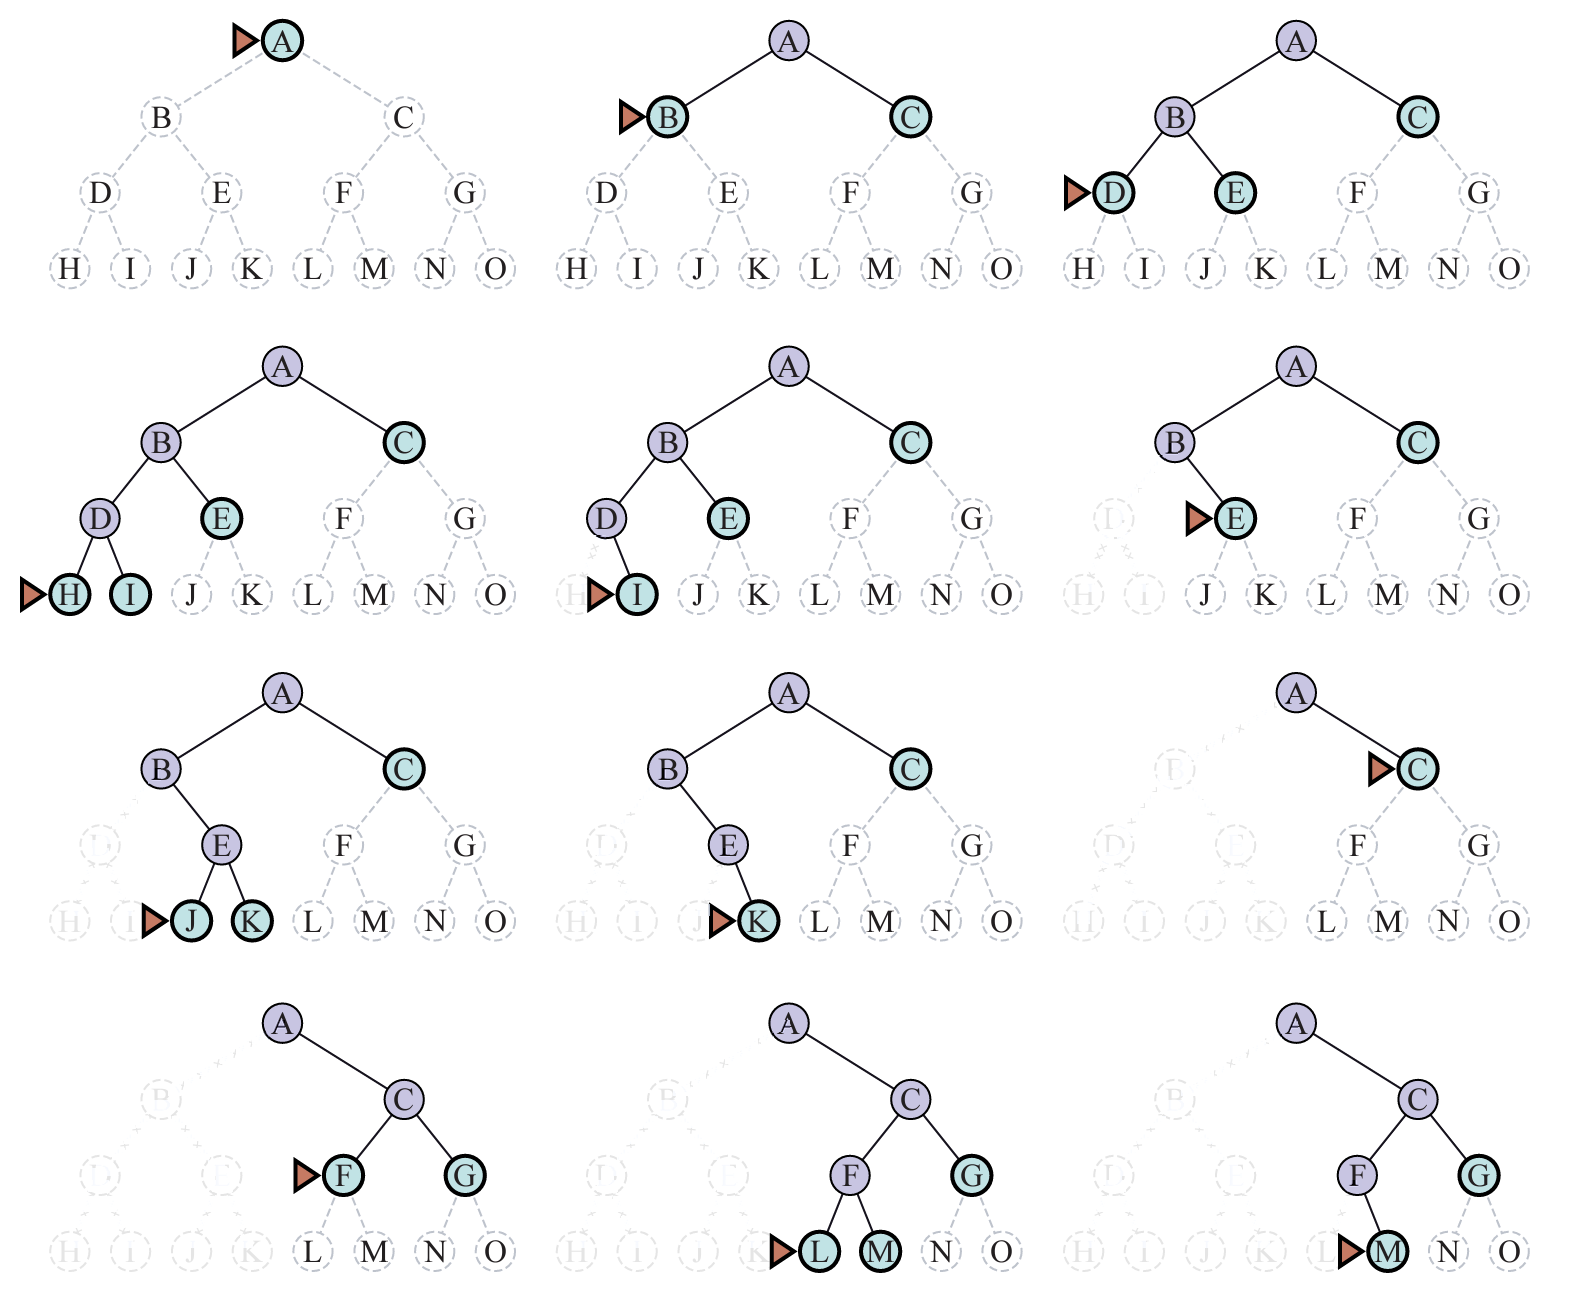
\includegraphics[scale=0.22]{./img/Profundidad}
\end{figure}

\end{frame}

%%%%%%%%%%%%%%%%%%%%%%%%%%%%%%%%

\begin{frame} \frametitle{Profundidad (Depth)} \footnotesize
\begin{itemize}
\item La búsqueda procesa inmediatamente el nivel más profundo del árbol, donde los nodos no tienen sucesores. La búsqueda vuelve al siguiente nivel más profundo que todavía no expandido los sucesores.

\item La búsqueda en profundidad no es óptima en coste ya que devuelve la primera solución incluso si no es la más barata.

\item La ventaja que aporta este algoritmo es la necesidad de menos memoria que los algoritmos vistos hasta ahora.

\item \textbf{Backtracking} es una variación que utiliza aún menos memoria, ya que solamente se genera un sucesor en vez de todos los sucesores.

\item El algoritmo no es completo, ya que el algoritmo puede caer un camino infinito en un espacio de estado infinito.

\end{itemize}


\end{frame}

%%%%%%%%%%%%%%%%%%%%%%%%%%%%%%%%
\begin{frame} \frametitle{Ejemplo Grafo - Profundidad} \scriptsize



\begin{columns}
\begin{column}{0.6\textwidth}

    \begin{center}
     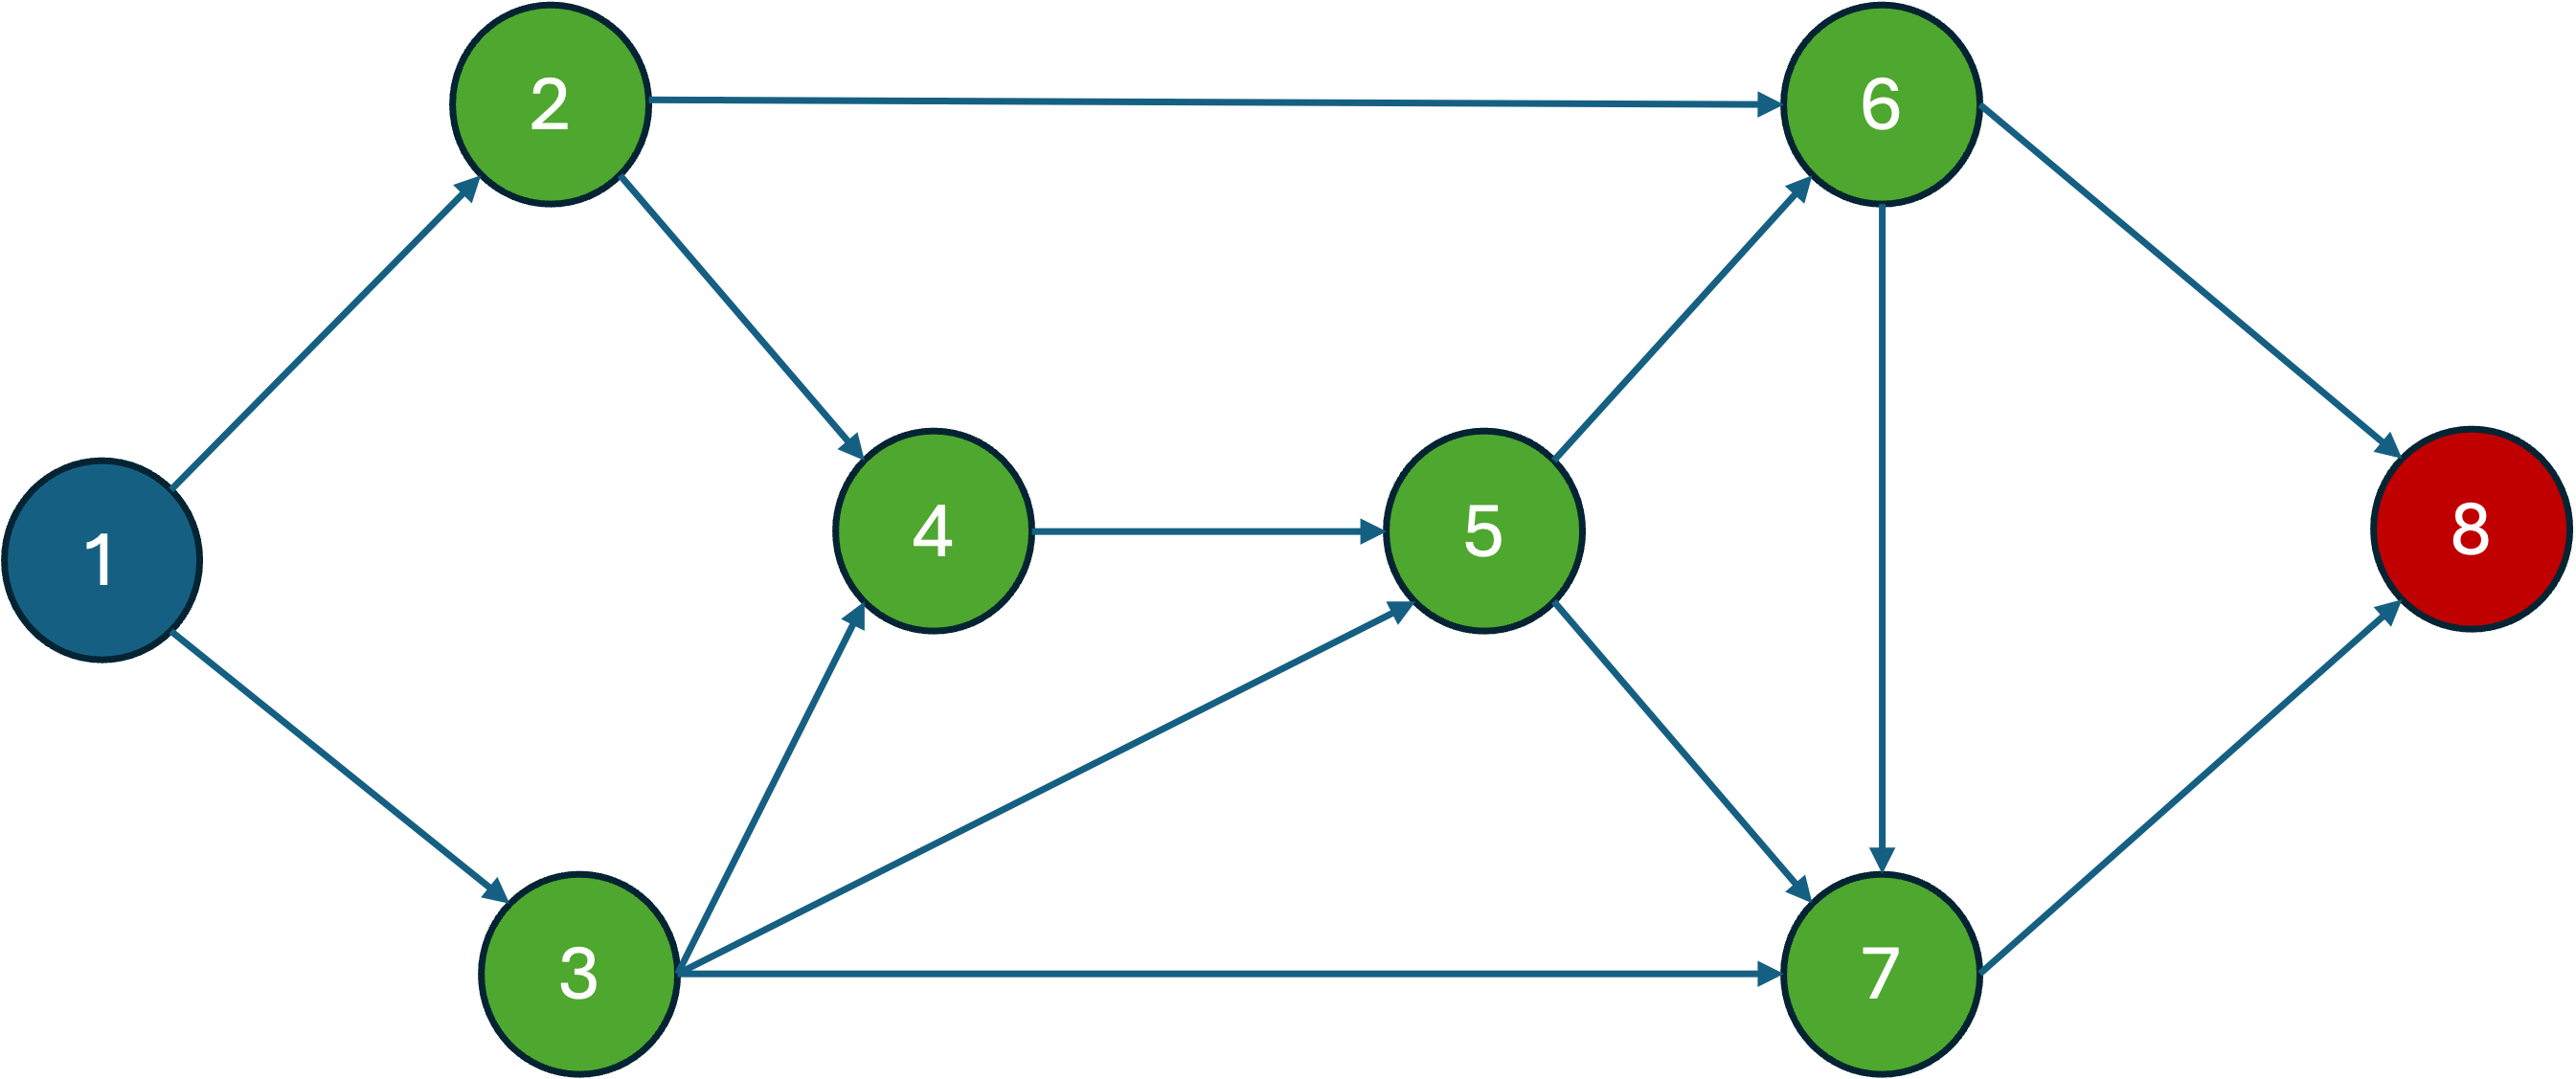
\includegraphics[width=0.6\textwidth]{img/GrafoEjemplo1}
     \end{center}
     
\begin{itemize}\scriptsize
    \item Nodo 1 - Expando nodo 1 - (2,3) Frontera: 2, 3\\
    \item Nodo 2 - Expando nodo 2 - (4,6) Frontera: 4, 6, 3\\
    \item Nodo 4 - Expando nodo 4 - (5) Frontera:  5, 6, 3\\
    \item Nodo 5 - Expando nodo 5 - (6,7) Frontera: 7, 6, 3 (6 Repetido)\\
    \item Nodo 7 - Expando nodo 7 - (8) Frontera: 8, 6, 3\\
    \item 8 SOL\\
\end{itemize}


\end{column}
\begin{column}{0.4\textwidth}  
    \begin{center}
      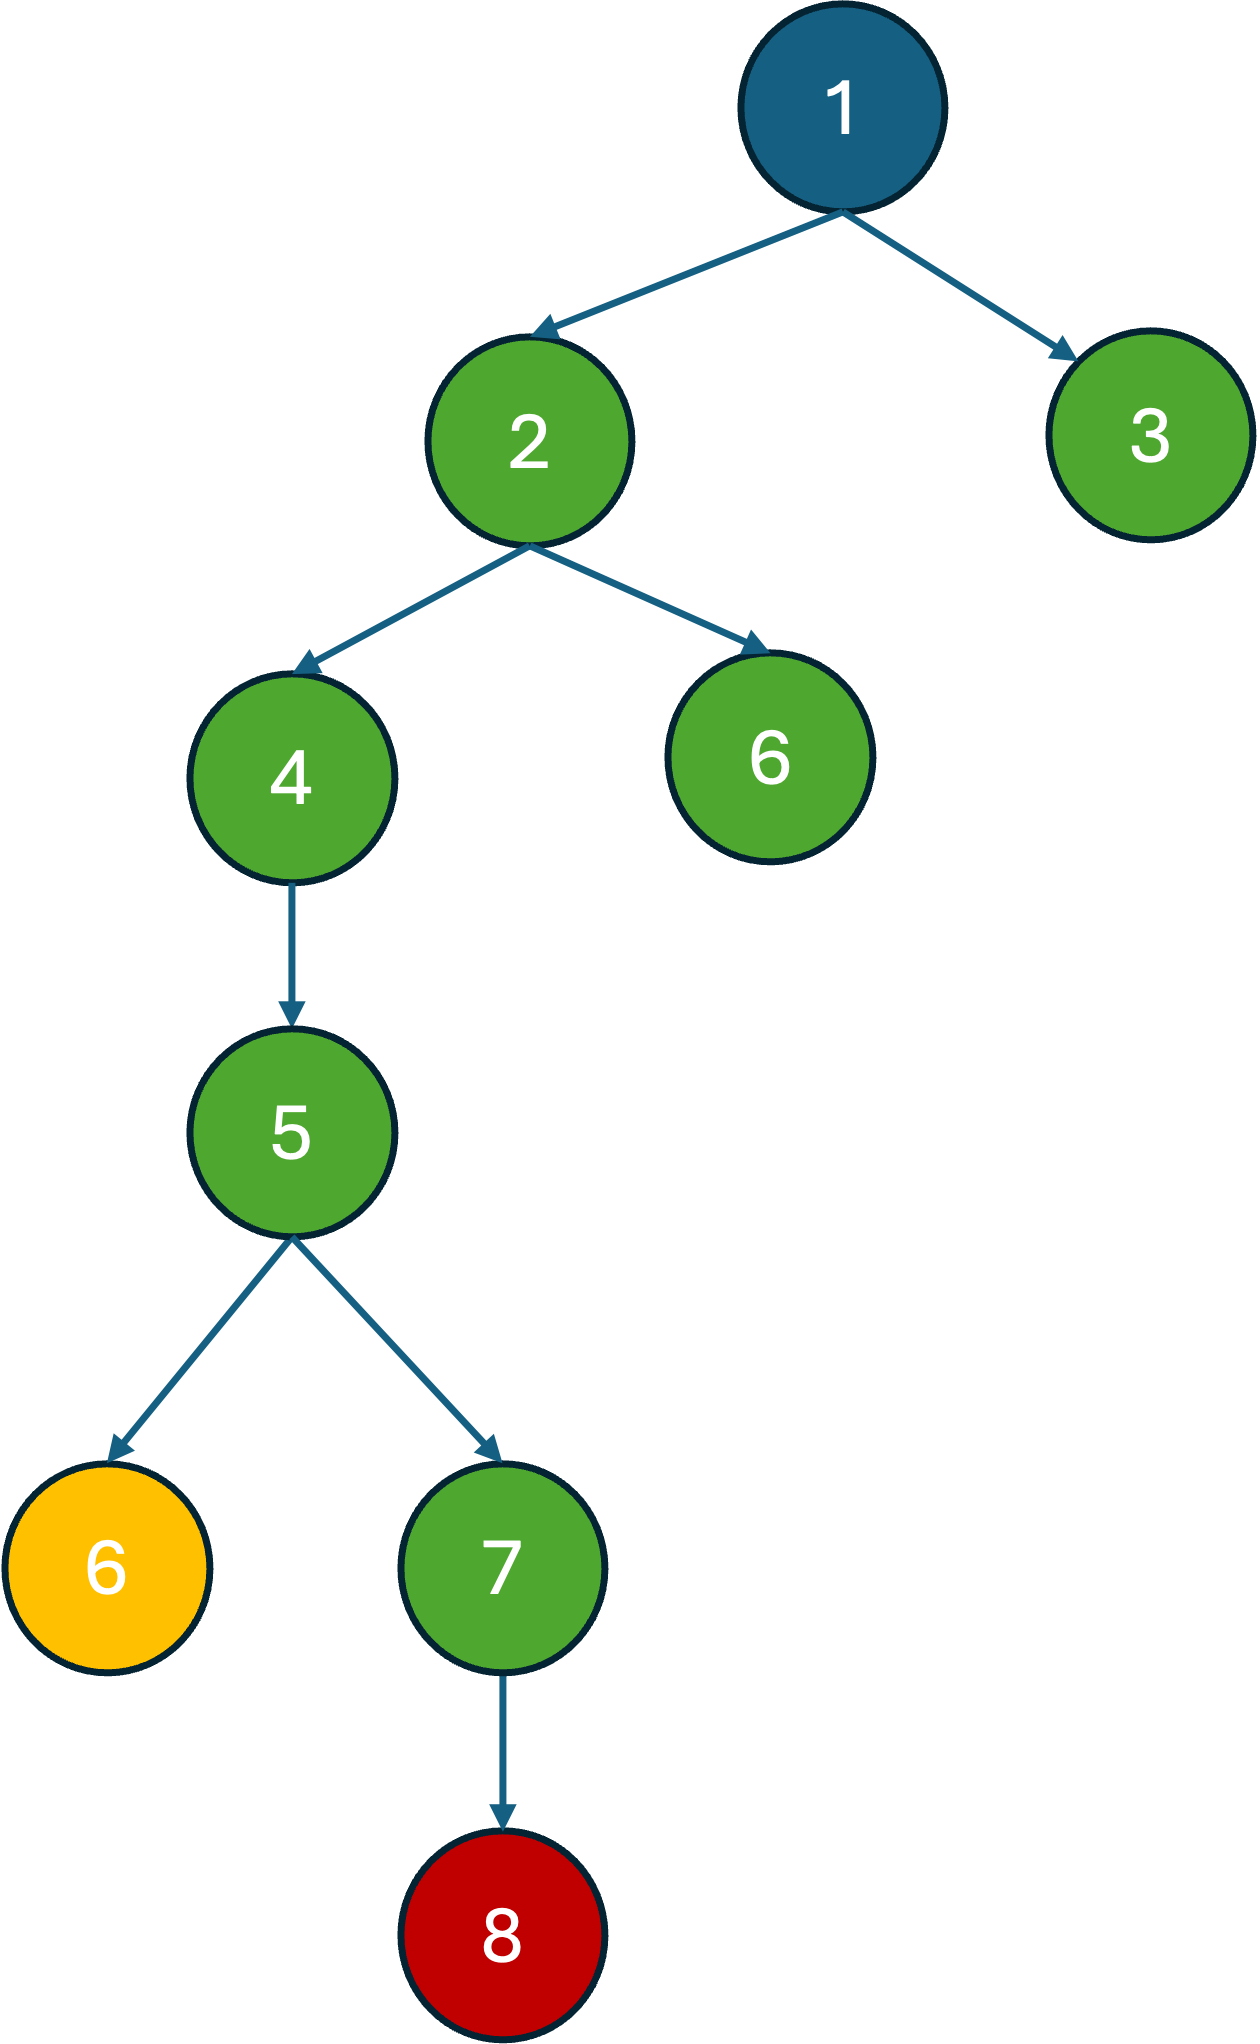
\includegraphics[width=0.6\textwidth]{img/ArbolProfundidad.png}
     \end{center}
\end{column}
\end{columns}


\end{frame} 
%%%%%%%%%%%%%%%%%%%%%%%%%%%%%%%%

%%%%%%%%%%%%%%%%%%%%%%%%%%%%%%%%
\begin{frame} [fragile ]\frametitle{Profundidad  en Python } \footnotesize
\begin{minted}[fontsize=\tiny]{python}
def depth_first_search(problem):
    reached = set()
    stack = [Node(problem.initial_state)]

    while stack:
        node = stack.pop()
        print (f"NODO SELECCIONADO {node}")
        if problem.is_goal(node.state):
            return node
        if tuple(node.state) not in reached:
            reached.add(tuple(node.state))
            children = [Node(child_state, node) for child_state in problem.expand(node.state)]
            stack.extend(children)
            imprimirFrontera(stack)

    return None
\end{minted}

\end{frame} 

%%%%%%%%%%%%%%%%%%%%%%%%%%%%%%%%
\begin{frame} [fragile ]\frametitle{Profundidad  en Python } \footnotesize
\begin{minted}[fontsize=\small]{python}

initial_state = '1'
goal_state = '8'
problem = ProblemGrafo(initial_state, goal_state)
solution_node = depth_first_search(problem)
\end{minted}

\end{frame} 


%%%%%%%%%%%%%%%%%%%%%%%%%%%%%%%%
%%%%%%%%%%%%%%%%%%%%%%%%%%%%%%%%
\subsection{Profundidad Limitada}
\begin{chapter}[images/etsiinformatica4.png]{uicblue}{Profundidad Limitada}
\end{chapter}

%%%%%%%%%%%%%%%%%%%%%%%%%%%%%%%%

\begin{frame} \frametitle{Profundidad  Limitada} \small
\begin{itemize}
\item Evitamos el problema de árboles ilimitados, estableciendo un límite de profundidad l predeterminado.

	\begin{itemize}
	\item Nodos a profundidad l se les trata como si no tuviesen sucesor.
	\end{itemize}

\item Incompletitud si $l < d,$ objetivo fuera alcance del límite profundidad. 
\end{itemize}


\begin{figure}
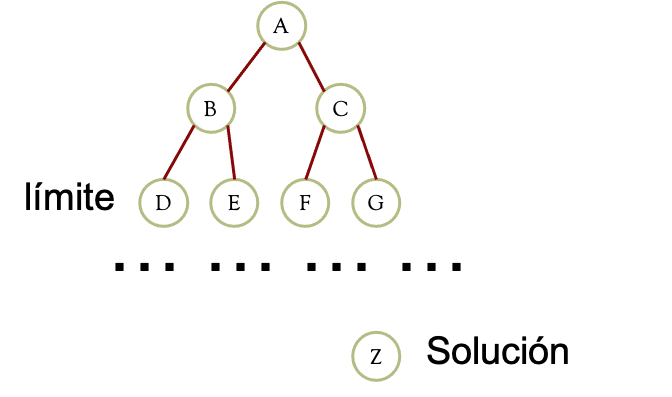
\includegraphics[scale=0.45]{./img/ProfundidadLimitada}
\end{figure}

\end{frame} 


%%%%%%%%%%%%%%%%%%%%%%%%%%%%%%%%
%%%%%%%%%%%%%%%%%%%%%%%%%%%%%%%%


\begin{frame} \frametitle{Profundidad Limitada} \footnotesize


\begin{figure}
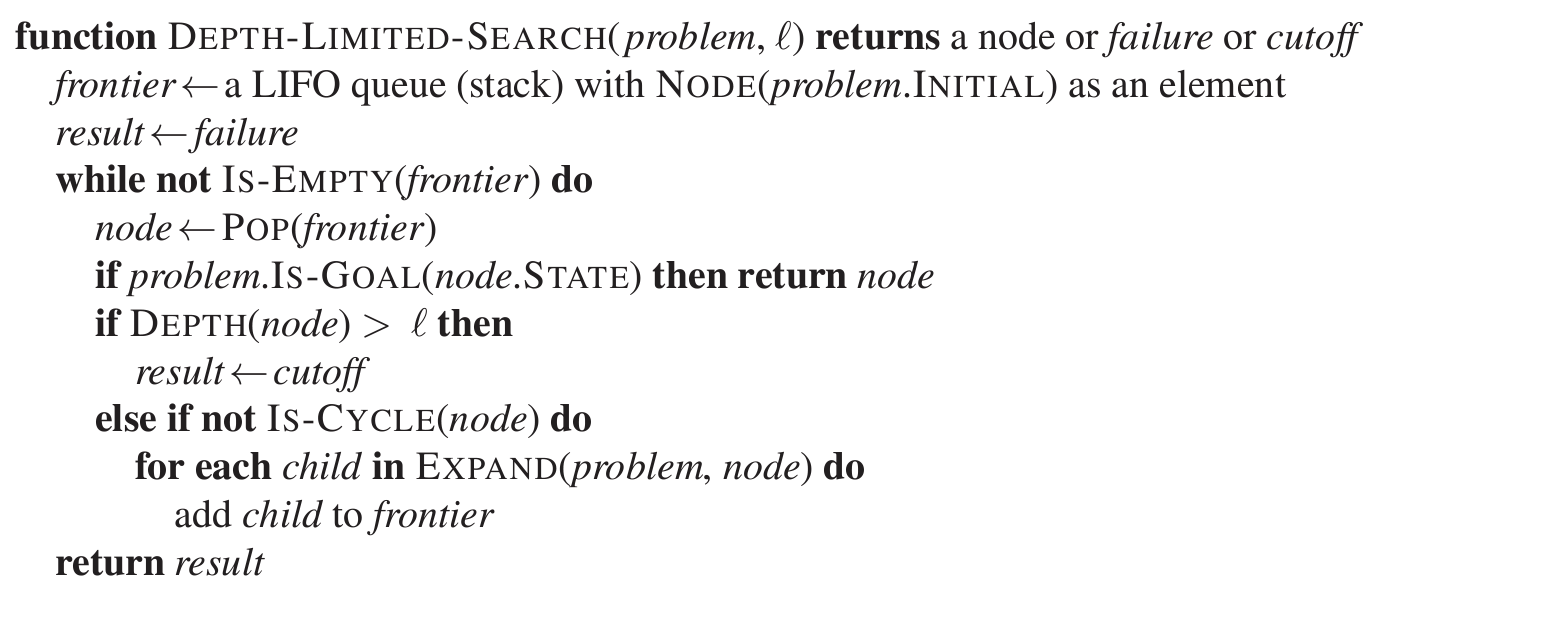
\includegraphics[scale=0.5]{./img/Depth-limited}
\end{figure}

\end{frame}
%%%%%%%%%%%%%%%%%%%%%%%%%%%%%%%%
%%%%%%%%%%%%%%%%%%%%%%%%%%%%%%%%
%%%%%%%%%%%%%%%%%%%%%%%%%%%%%%%%
\subsection{Profundidad Progresiva}
\begin{chapter}[images/etsiinformatica4.png]{uicblue}{Profundidad Progresiva}
\end{chapter}

%%%%%%%%%%%%%%%%%%%%%%%%%%%%%%%%


%%%%%%%%%%%%%%%%%%%%%%%%%%%%%%%%

\begin{frame} \frametitle{Profundidad  Progresiva o Iterativa} \small

\begin{itemize}
\item La profundidad progresiva es el método de búsqueda no informada elegido cuando el espacio de búsqueda no puede ser almacenado en la memoria y la profundidad de la solución no es conocida.

\end{itemize}
\begin{figure}
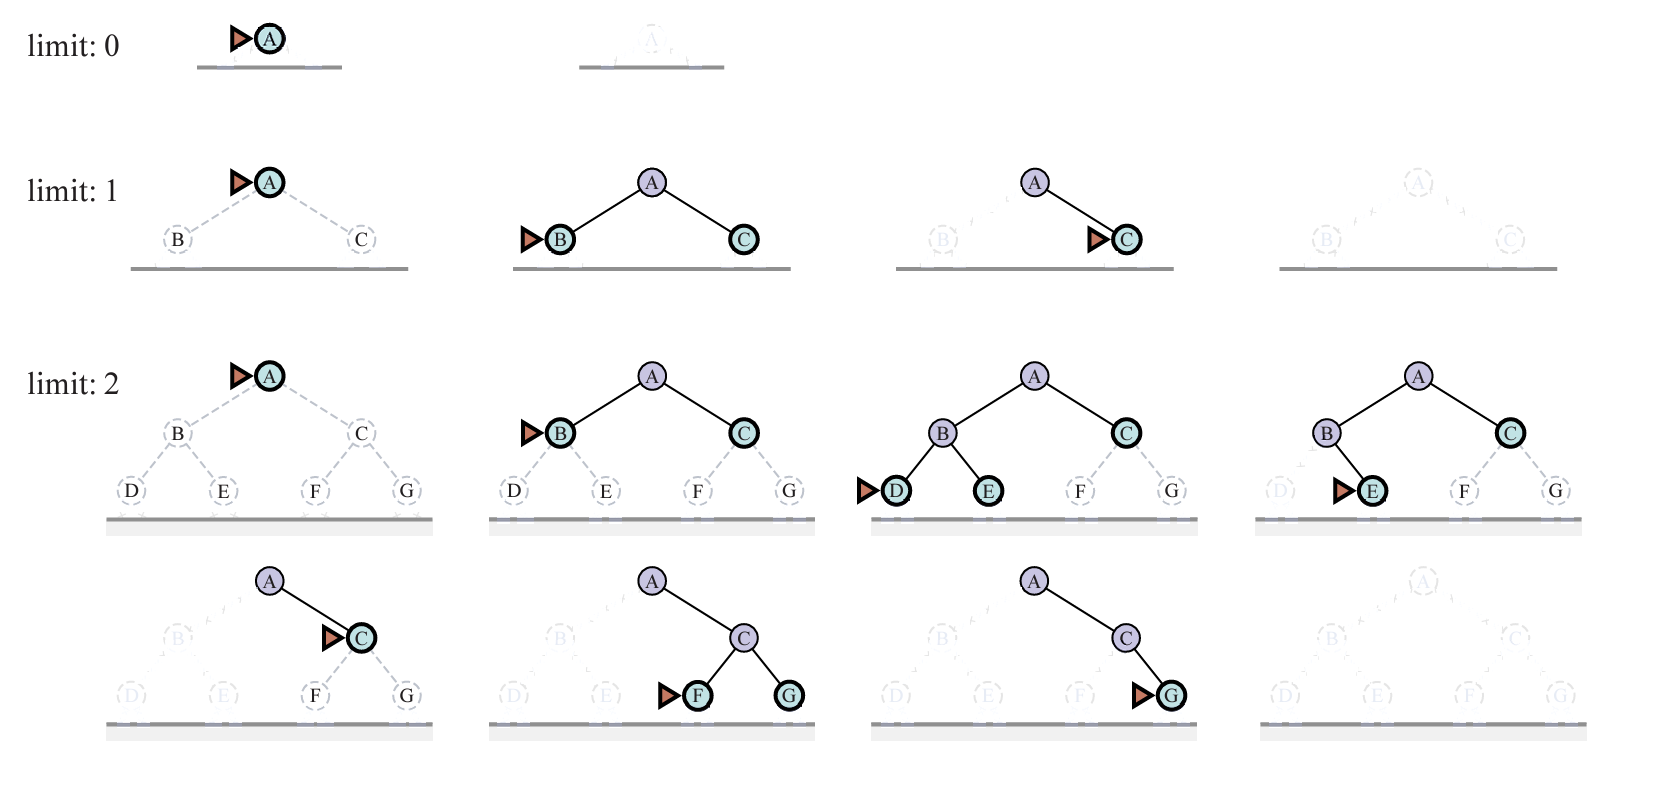
\includegraphics[scale=0.33]{./img/profundidadlimitada1}
\end{figure}

\end{frame} 

%%%%%%%%%%%%%%%%%%%%%%%%%%%%%%%%

\begin{frame} \frametitle{Profundidad  Progresiva o Iterativa} \small

\begin{figure}
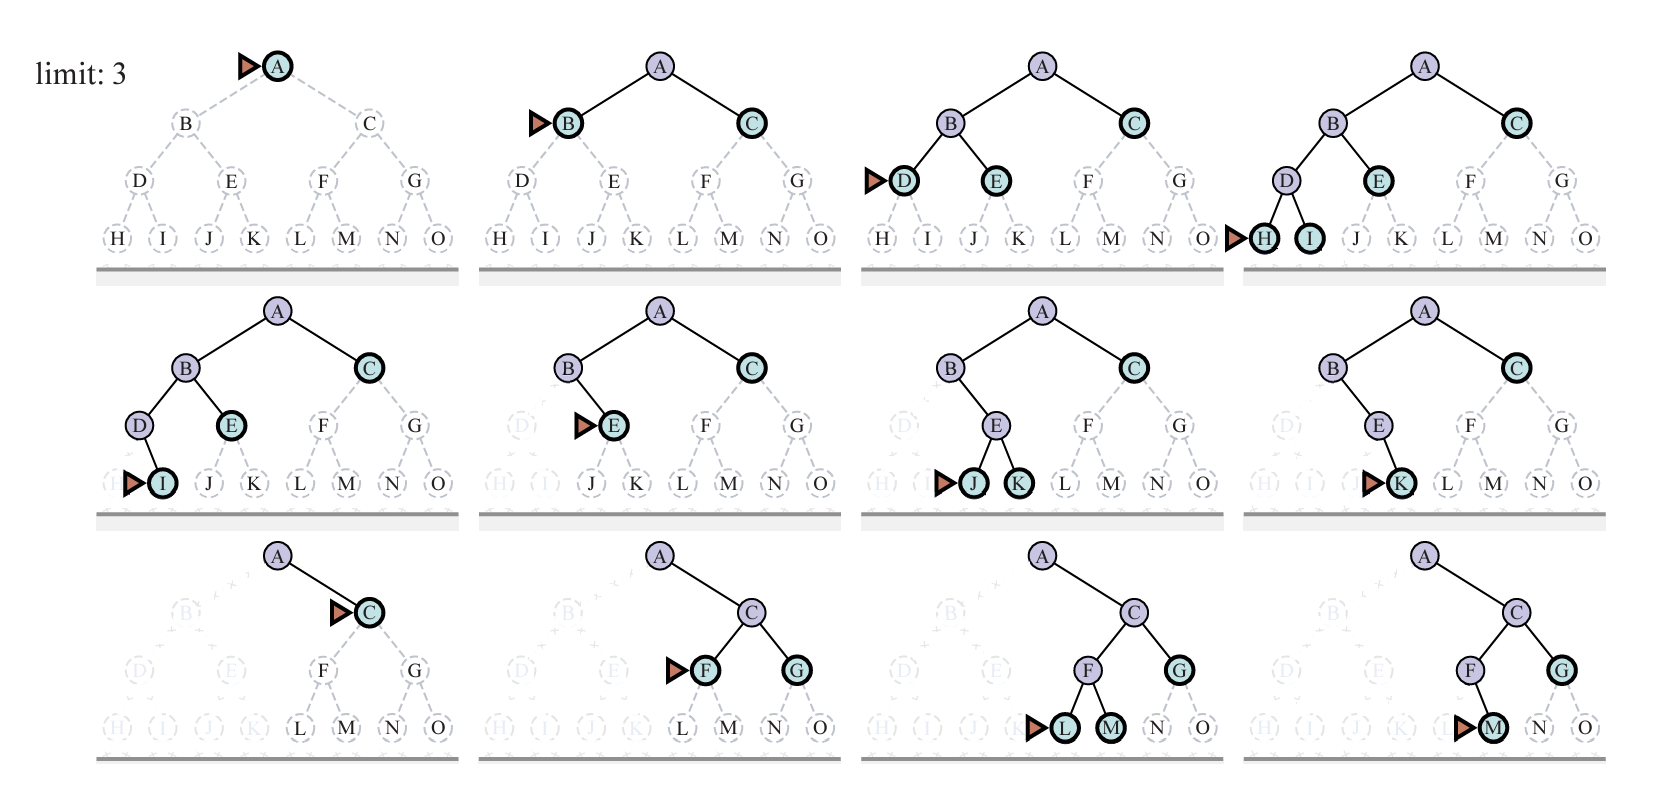
\includegraphics[scale=0.45]{./img/profundidadlimitada2}
\end{figure}

\end{frame} 
%%%%%%%%%%%%%%%%%%%%%%%%%%%%%%%%

\begin{frame} \frametitle{Profundidad  Progresiva o Iterativa} \small

\begin{figure}
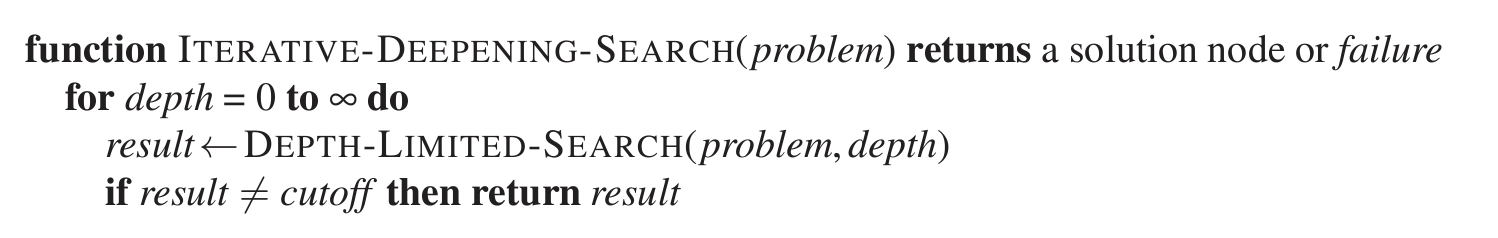
\includegraphics[scale=0.45]{./img/iterative}
\end{figure}

\end{frame} 

%%%%%%%%%%%%%%%%%%%%%%%%%%%%%%%%

\begin{frame} \frametitle{Ejemplo Grafo - Profundidad  Progresiva o Iterativa} \small

\begin{figure}
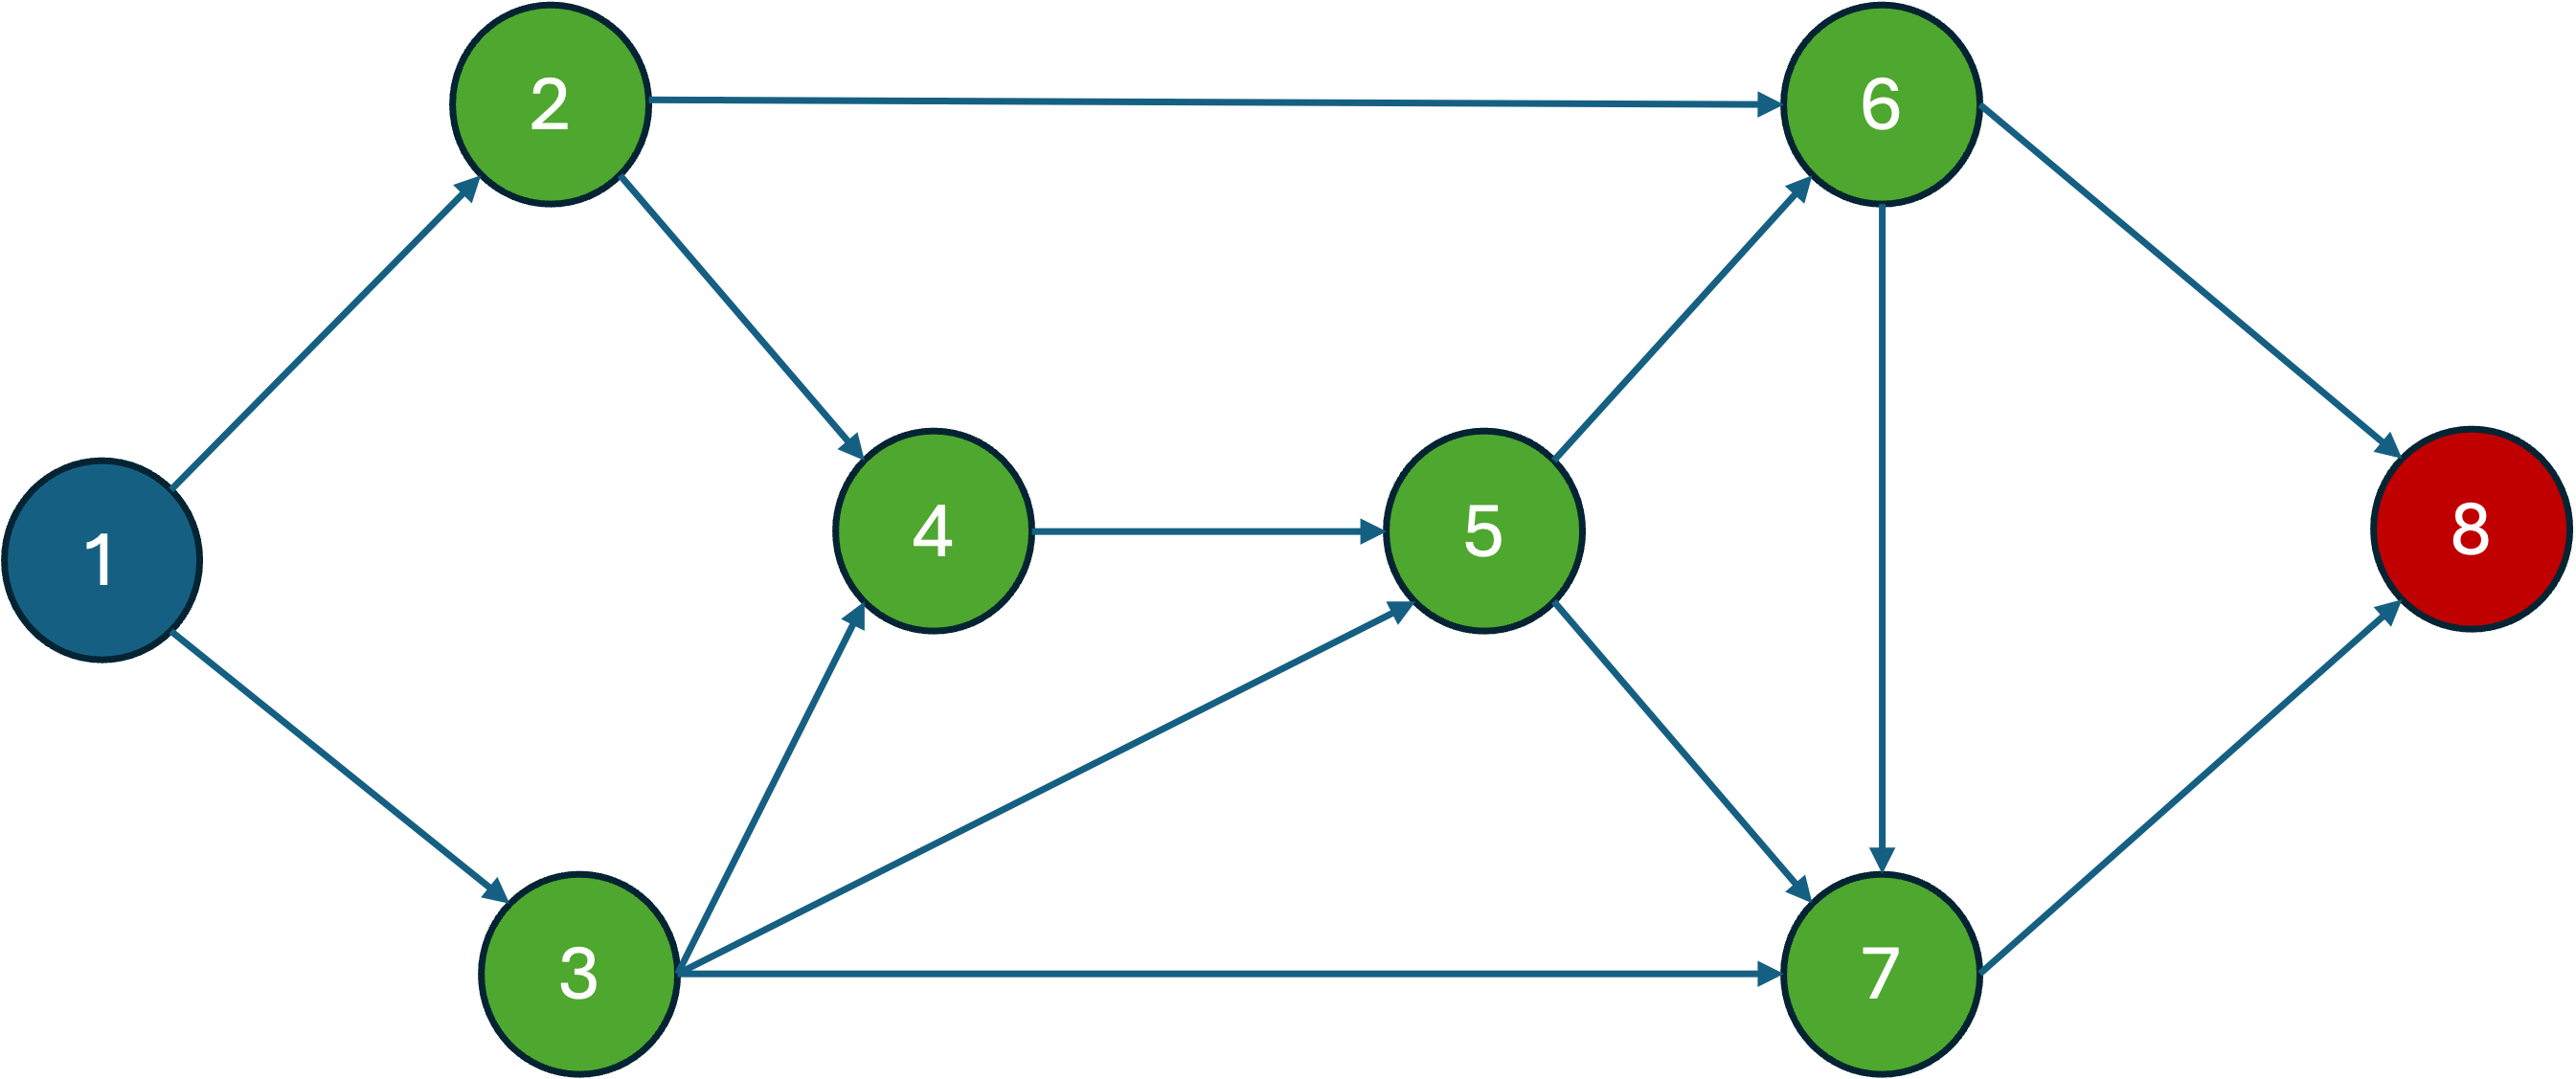
\includegraphics[scale=0.45]{./img/GrafoEjemplo1}
\end{figure}

\end{frame} 
%%%%%%%%%%%%%%%%%%%%%%%%%%%%%%%%
\begin{frame} \frametitle{Ejemplo Grafo - Profundidad  Progresiva o Iterativa} \scriptsize



\begin{columns}
\begin{column}{0.7\textwidth}

\begin{itemize}
    \item - \textbf{Profundidad 1}

        \begin{itemize}\scriptsize
        \item Nodo 1. Expando nodo 1 - Fuera Limite - Frontera
        \end{itemize}
   
    \item - \textbf{Profundidad 2}

        \begin{itemize}\scriptsize
            \item Nodo 1. Expando nodo 1 -  (2,3) - Frontera 2, 3.
            \item Nodo 2. Expando nodo 2 - Fuera Limite - Frontera 3.
            \item Nodo 2. Expando nodo 3 - Fuera Limite - Frontera .
        \end{itemize}

    \item - \textbf{Profundidad 3}

        \begin{itemize}\scriptsize
            \item Nodo 1. Expando nodo 1 -  (2,3) - Frontera 2, 3.
            \item Nodo 2. Expando nodo 2 - (4,6) - Frontera 4,6,3.
            \item Nodo 4. Expando nodo 4 - Fuera Limite - Frontera 6,3.
            \item Nodo 6. Expando nodo 6 - Fuera Limite - Frontera 3.
            \item Nodo 3. Expando nodo 3 - (4,5,7) - Frontera 5,7. (4 Repetido)
            \item Nodo 5. Expando nodo 5 - Fuera Limite - Frontera 7.
            \item Nodo 7.  Expando nodo 7 - Fuera Limite - Frontera .
        \end{itemize}

    
\end{itemize}

    


\end{column}
\begin{column}{0.4\textwidth}  
    \begin{center}
      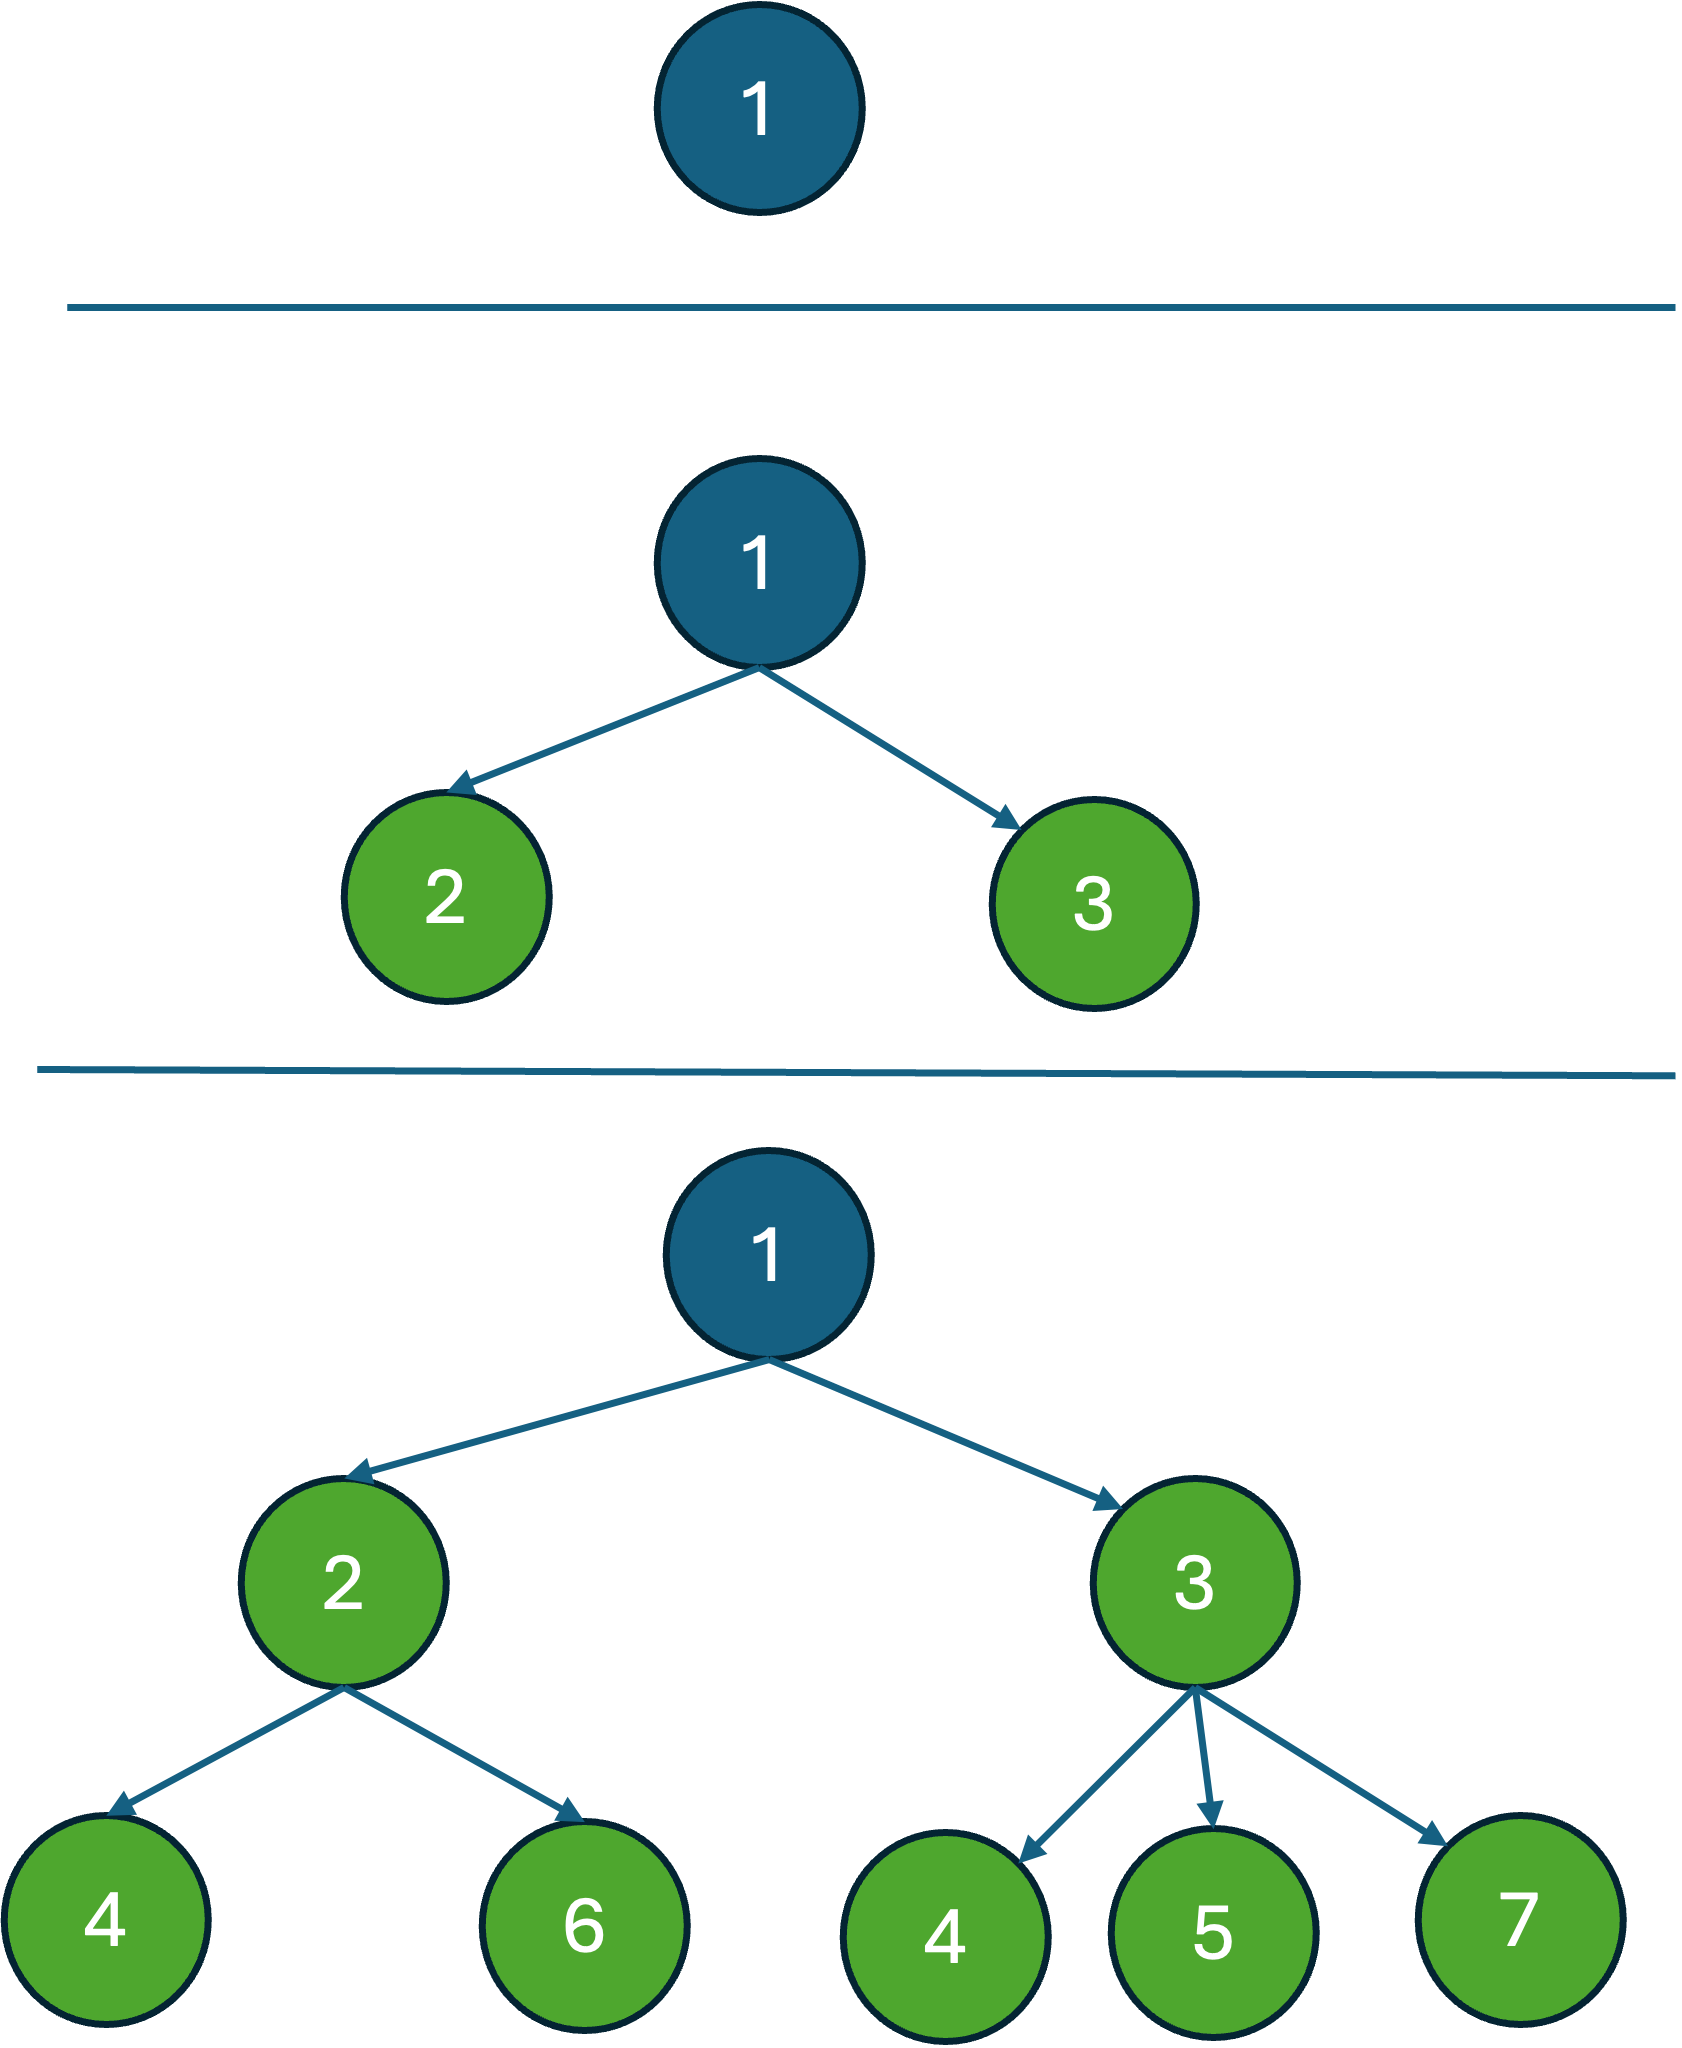
\includegraphics[width=0.6\textwidth]{img/Nivel1-3.png}
     \end{center}
\end{column}
\end{columns}


\end{frame} 


%%%%%%%%%%%%%%%%%%%%%%%%%%%%%%%%
\begin{frame} \frametitle{Ejemplo Grafo - Profundidad  Progresiva o Iterativa} \scriptsize



\begin{columns}
\begin{column}{0.7\textwidth}

\begin{itemize}
    \item - \textbf{Profundidad 4}

        \begin{itemize}\scriptsize
            \item Nodo 1. Expando nodo 1 -  (2,3) - Frontera 2, 3.
            \item Nodo 2. Expando nodo 2 - (4,6) - Frontera 4,6,3.
            \item Nodo 4. Expando nodo 4 - 5 - Frontera 5,6,3.
            \item Nodo 6. Expando nodo 5 - Fuera Limite - Frontera 6,3.
            \item Nodo 3. Expando nodo 6 - (7,8) - Frontera 7,8,3.
            \item Nodo 5. Expando nodo 5 - Fuera Limite - Frontera 8,3.
            \item Nodo 8. Expando nodo 8 - Solución - Frontera 3.
        \end{itemize}
\end{itemize}

    


\end{column}
\begin{column}{0.4\textwidth}  
    \begin{center}
      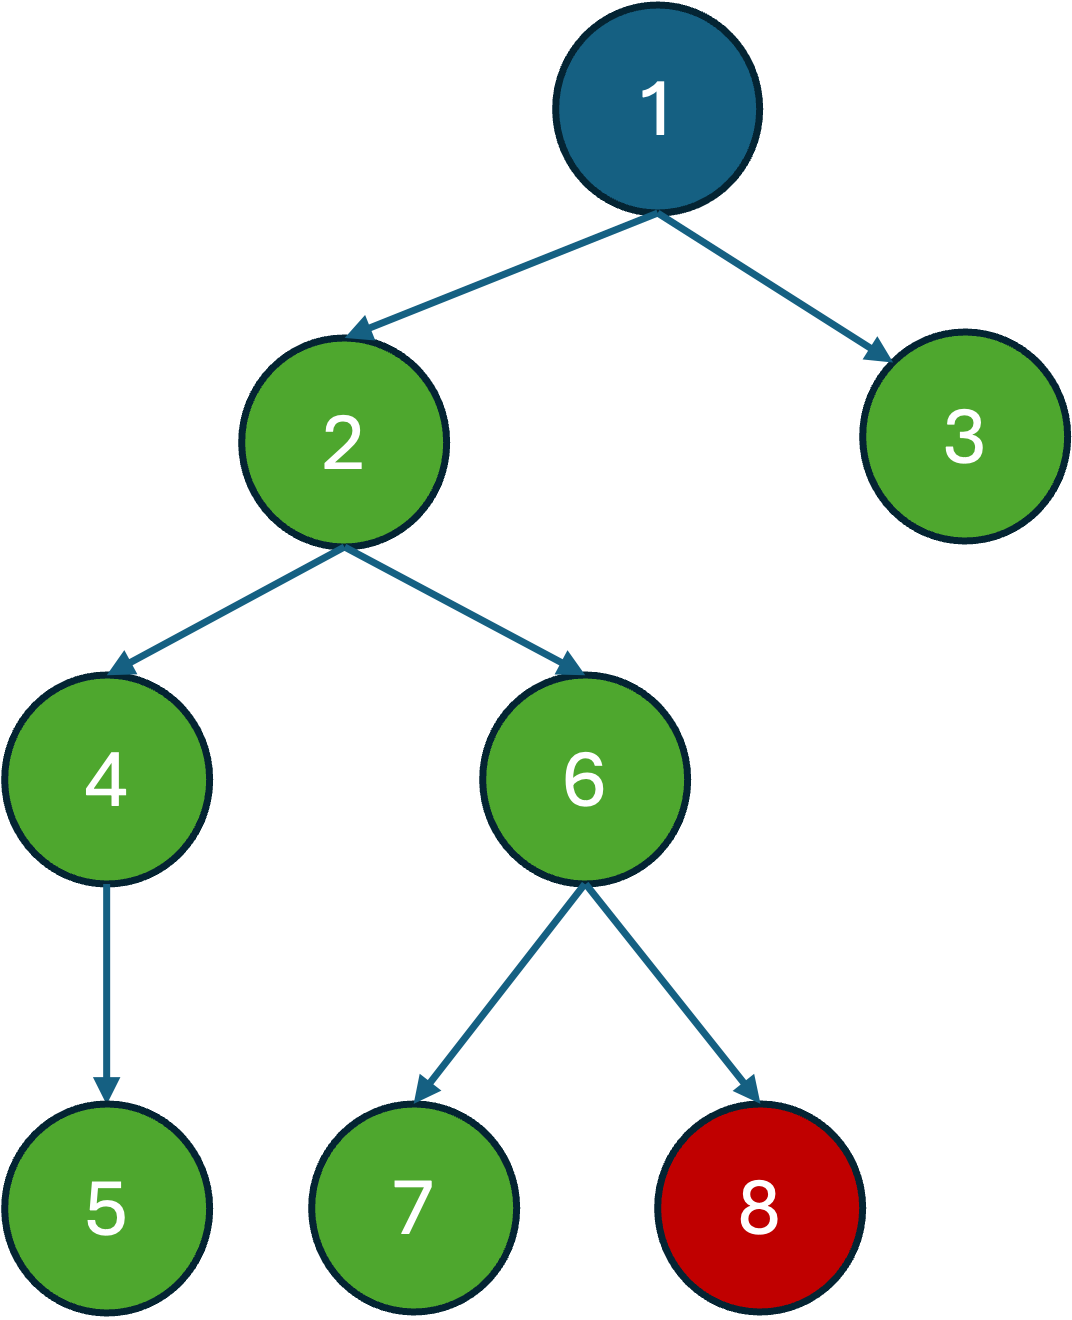
\includegraphics[width=0.6\textwidth]{img/Nivel4.png}
     \end{center}
\end{column}
\end{columns}


\end{frame} 
%%%%%%%%%%%%%%%%%%%%%%%%%%%%%%%%
%%%%%%%%%%%%%%%%%%%%%%%%%%%%%%%%
%%%%%%%%%%%%%%%%%%%%%%%%%%%%%%%%
\subsection{Búsqueda Bidireccional}
\begin{chapter}[images/etsiinformatica4.png]{uicblue}{Búsqueda Bidireccional}
\end{chapter}

%%%%%%%%%%%%%%%%%%%%%%%%%%%%%%%%

\begin{frame} \frametitle{Búsqueda Bidireccional} \small
\begin{itemize}
    \item  Realiza la búsqueda iniciando tanto desde el estado inicial como de los estados finales, con la esperanza que las búsquedas se encuentren.

    \item La motivación es la complejidad ya que $b^{d/2} + b^{d/2}$ es menor que $b^{d}$.

    \item El algoritmo mantiene dos estructuras de fronteras y de estados alcanzados.
    Cuando un camino en una frontera alcanza un estado que también ha sido alcanzado en la otra mitad de la búsqueda, los dos caminos son unificados para establecer una solución.

    \item La primera solución que obtenemos no es garantizada que sea la mejor, la función TERMINATED determinará cuando parar de buscar nuevas soluciones.
\end{itemize}

\end{frame} 
%%%%%%%%%%%%%%%%%%%%%%%%%%%%%%%%

\begin{frame} \frametitle{Búsqueda Bidireccional} \footnotesize

\begin{columns}

\begin{column}{0.6\textwidth}  
    \begin{center}
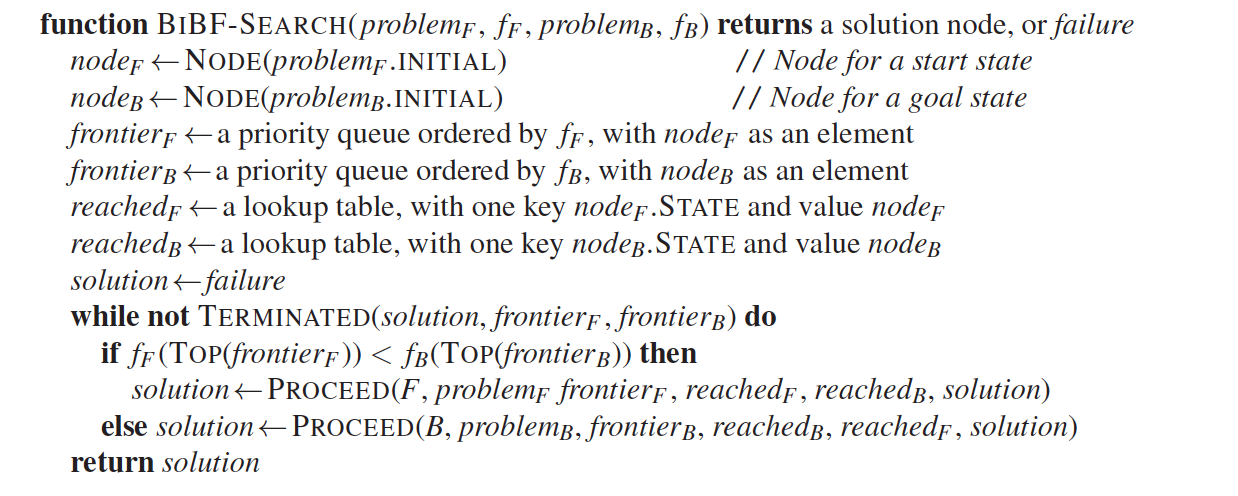
\includegraphics[scale=0.2]{./img/BIBF1}
     \end{center}
\end{column}

\begin{column}{0.4\textwidth}\scriptsize

Pasamos dos versiones del problema y la función de evaluación, una en la dirección hacia delante (subíndice F) y otra hacia atrás (subíndice B).\\
\vspace{0.3cm}
Necesitamos llevar la cuenta de dos fronteras y dos tablas de estados alcanzados,
y necesitamos ser capaces de razonar hacia atrás.\\
\vspace{0.3cm}

\end{column}

\end{columns}

\end{frame} 

%%%%%%%%%%%%%%%%%%%%%%%%%%%%%%%%

\begin{frame} \frametitle{Búsqueda Bidireccional} \footnotesize

\begin{columns}

\begin{column}{0.6\textwidth}  
    \begin{center}
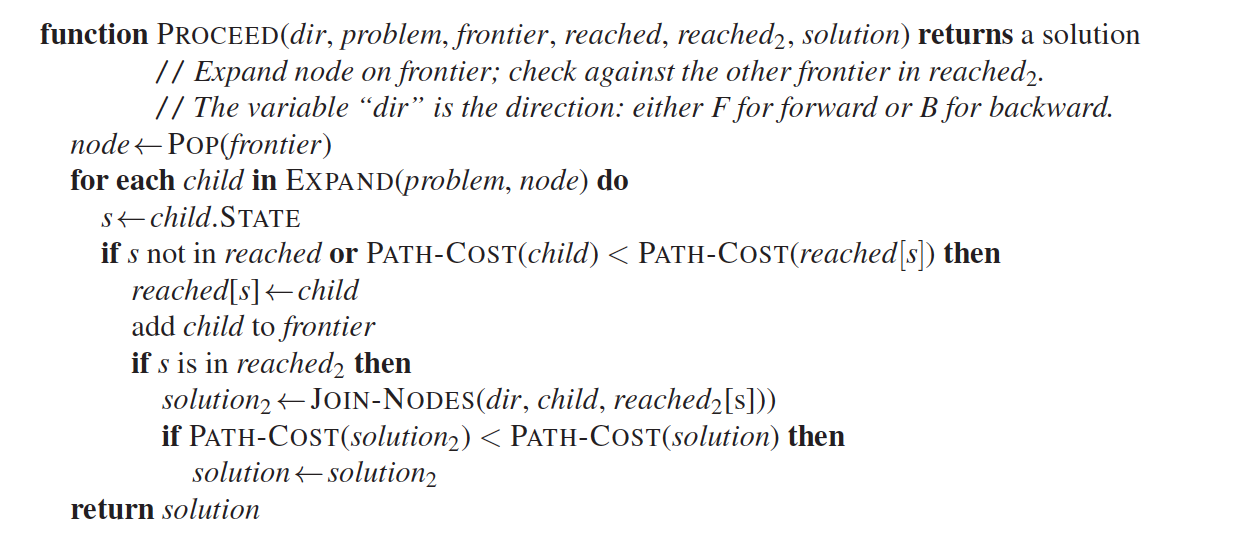
\includegraphics[scale=0.2]{./img/PROCEED}
     \end{center}
\end{column}

\begin{column}{0.4\textwidth}\scriptsize

si el estado s' es un sucesor de s en la dirección hacia adelante, entonces necesitamos saber que s es un sucesor de s' en la dirección hacia atrás.\\
\vspace{0.3cm}
Cuando un camino de una frontera alcanza un estado que también se alcanzó en la otra mitad de la búsqueda, los dos caminos se unen (mediante la función JOIN-NODES) para formar una solución.\\
\vspace{0.3cm}
Tenemos una solución cuando las dos fronteras chocan.

\end{column}

\end{columns}

\end{frame} 

%%%%%%%%%%%%%%%%%%%%%%%%%%%%%%%%
%%%%%%%%%%%%%%%%%%%%%%%%%%%%%%%%
%%%%%%%%%%%%%%%%%%%%%%%%%%%%%%%%
\subsection{Comparativa}
\begin{chapter}[images/etsiinformatica4.png]{uicblue}{Comparativa}
\end{chapter}


 %%%%%%%%%%%%%%%%%%%%%%%%%%%%%%%%

\begin{frame} \frametitle{Comparativa} \tiny

\begin{figure}
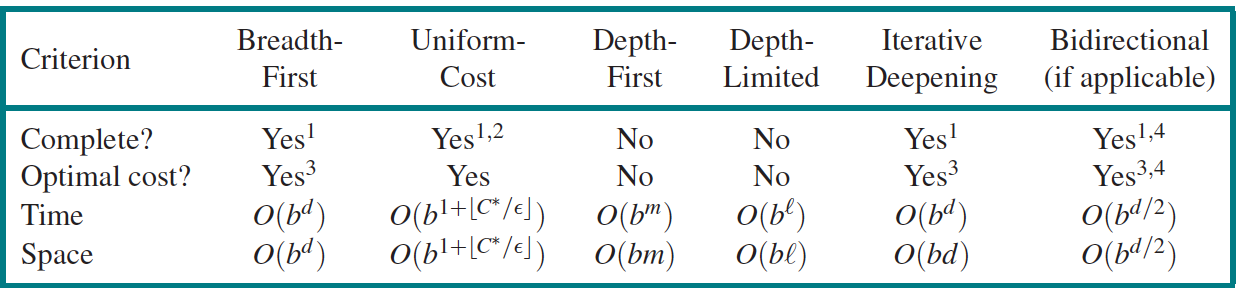
\includegraphics[scale=0.5]{./img/TablaComparativa}
\end{figure}

\begin{itemize}\tiny
    \item b es el factor de ramificación.
    \item m es la máxima profundidad del árbol de búsqueda.
    \item d es la profundidad de la solución menos profunda, o es m cuando no hay solución
    \item d is the depth of the shallowest solution, or is m when there is no solution;
    \item l es límite de profundidad.
\end{itemize}

\begin{itemize}\tiny
    \item 1 completo si b es finitio, y el espacionde estado tiene solución o es finito.e.
    \item 2 completo si los costes de todas las acciones $\geq \epsilon  > 0$;
    \item 3 coste óptimo si el coste de todas las acciones son idénticas;
    \item 4 si ambas direcciones son aplicando alguritmo de amplitud o con coste uniforme.
\end{itemize}
\end{frame} 


%%%%%%%%%%%%%%%%%%%%%%%%%%%%%%%%
%\begin{frame}  \small  
%\end{frame} 


%%%%%%%%%%%%%%%%%%%%%%%%%%%%%%%%
%\begin{frame}  \small  
%\end{frame} 


%%%%%%%%%%%%%%%%%%%%%%%%%%%%%%%%
%\begin{frame}  \small  
%\end{frame} 


%%%%%%%%%%%%%%%%%%%%%%%%%%%%%%%%
%\begin{frame}  \small  
%\end{frame} 

%%%%%%%%%%%%%%%%%%%%%%%%%%%%%%%%
%%%%%%%%%%%%%%%%%%%%%%%%%%%%%%%%

%%%%%%%%%%%%%%%%%%%%%%%%%%%%%%%%
%%%%%%%%%%%%%%%%%%%%%%%%%%%%%%%%
   
\backmatter


\end{document}